\documentclass[nofonts,]{tufte-handout}

% ams
\usepackage{amssymb,amsmath}

\usepackage{ifxetex,ifluatex}
\usepackage{fixltx2e} % provides \textsubscript
\ifnum 0\ifxetex 1\fi\ifluatex 1\fi=0 % if pdftex
  \usepackage[T1]{fontenc}
  \usepackage[utf8]{inputenc}
\else % if luatex or xelatex
  \makeatletter
  \@ifpackageloaded{fontspec}{}{\usepackage{fontspec}}
  \makeatother
  \defaultfontfeatures{Ligatures=TeX,Scale=MatchLowercase}
  \makeatletter
  \@ifpackageloaded{soul}{
     \renewcommand\allcapsspacing[1]{{\addfontfeature{LetterSpace=15}#1}}
     \renewcommand\smallcapsspacing[1]{{\addfontfeature{LetterSpace=10}#1}}
   }{}
  \makeatother
\fi

% graphix
\usepackage{graphicx}
\setkeys{Gin}{width=\linewidth,totalheight=\textheight,keepaspectratio}

% booktabs
\usepackage{booktabs}

% url
\usepackage{url}

% hyperref
\usepackage{hyperref}

% units.
\usepackage{units}


\setcounter{secnumdepth}{-1}

% citations

%% tint override
\setcitestyle{round} 

% pandoc syntax highlighting
\usepackage{color}
\usepackage{fancyvrb}
\newcommand{\VerbBar}{|}
\newcommand{\VERB}{\Verb[commandchars=\\\{\}]}
\DefineVerbatimEnvironment{Highlighting}{Verbatim}{commandchars=\\\{\}}
% Add ',fontsize=\small' for more characters per line
\usepackage{framed}
\definecolor{shadecolor}{RGB}{248,248,248}
\newenvironment{Shaded}{\begin{snugshade}}{\end{snugshade}}
\newcommand{\AlertTok}[1]{\textcolor[rgb]{0.94,0.16,0.16}{#1}}
\newcommand{\AnnotationTok}[1]{\textcolor[rgb]{0.56,0.35,0.01}{\textbf{\textit{#1}}}}
\newcommand{\AttributeTok}[1]{\textcolor[rgb]{0.13,0.29,0.53}{#1}}
\newcommand{\BaseNTok}[1]{\textcolor[rgb]{0.00,0.00,0.81}{#1}}
\newcommand{\BuiltInTok}[1]{#1}
\newcommand{\CharTok}[1]{\textcolor[rgb]{0.31,0.60,0.02}{#1}}
\newcommand{\CommentTok}[1]{\textcolor[rgb]{0.56,0.35,0.01}{\textit{#1}}}
\newcommand{\CommentVarTok}[1]{\textcolor[rgb]{0.56,0.35,0.01}{\textbf{\textit{#1}}}}
\newcommand{\ConstantTok}[1]{\textcolor[rgb]{0.56,0.35,0.01}{#1}}
\newcommand{\ControlFlowTok}[1]{\textcolor[rgb]{0.13,0.29,0.53}{\textbf{#1}}}
\newcommand{\DataTypeTok}[1]{\textcolor[rgb]{0.13,0.29,0.53}{#1}}
\newcommand{\DecValTok}[1]{\textcolor[rgb]{0.00,0.00,0.81}{#1}}
\newcommand{\DocumentationTok}[1]{\textcolor[rgb]{0.56,0.35,0.01}{\textbf{\textit{#1}}}}
\newcommand{\ErrorTok}[1]{\textcolor[rgb]{0.64,0.00,0.00}{\textbf{#1}}}
\newcommand{\ExtensionTok}[1]{#1}
\newcommand{\FloatTok}[1]{\textcolor[rgb]{0.00,0.00,0.81}{#1}}
\newcommand{\FunctionTok}[1]{\textcolor[rgb]{0.13,0.29,0.53}{\textbf{#1}}}
\newcommand{\ImportTok}[1]{#1}
\newcommand{\InformationTok}[1]{\textcolor[rgb]{0.56,0.35,0.01}{\textbf{\textit{#1}}}}
\newcommand{\KeywordTok}[1]{\textcolor[rgb]{0.13,0.29,0.53}{\textbf{#1}}}
\newcommand{\NormalTok}[1]{#1}
\newcommand{\OperatorTok}[1]{\textcolor[rgb]{0.81,0.36,0.00}{\textbf{#1}}}
\newcommand{\OtherTok}[1]{\textcolor[rgb]{0.56,0.35,0.01}{#1}}
\newcommand{\PreprocessorTok}[1]{\textcolor[rgb]{0.56,0.35,0.01}{\textit{#1}}}
\newcommand{\RegionMarkerTok}[1]{#1}
\newcommand{\SpecialCharTok}[1]{\textcolor[rgb]{0.81,0.36,0.00}{\textbf{#1}}}
\newcommand{\SpecialStringTok}[1]{\textcolor[rgb]{0.31,0.60,0.02}{#1}}
\newcommand{\StringTok}[1]{\textcolor[rgb]{0.31,0.60,0.02}{#1}}
\newcommand{\VariableTok}[1]{\textcolor[rgb]{0.00,0.00,0.00}{#1}}
\newcommand{\VerbatimStringTok}[1]{\textcolor[rgb]{0.31,0.60,0.02}{#1}}
\newcommand{\WarningTok}[1]{\textcolor[rgb]{0.56,0.35,0.01}{\textbf{\textit{#1}}}}

% longtable
\usepackage{longtable,booktabs}
\usepackage{array}

% multiplecol
\usepackage{multicol}

% strikeout
\usepackage[normalem]{ulem}

% morefloats
\usepackage{morefloats}


% tightlist macro required by pandoc >= 1.14
\providecommand{\tightlist}{%
  \setlength{\itemsep}{0pt}\setlength{\parskip}{0pt}}

% title / author / date
\title{Supplement 1: Analysing community change through time with palaeo
data}
\author{Olivia Rata Burge}
\date{Manaaki Whenua - Landcare Research}

%% -- tint overrides
%% fonts, using roboto (condensed) as default
\usepackage[sfdefault,condensed]{roboto}
%% also nice: \usepackage[default]{lato}

%% colored links, setting 'borrowed' from RJournal.sty with 'Thanks, Achim!'
\RequirePackage{color}
\definecolor{link}{rgb}{0.3,0.3,0.6} %% blue with some grey
\hypersetup{
  colorlinks,%
  citecolor=link,%
  filecolor=link,%
  linkcolor=link,%
  urlcolor=link
}

%% macros
\makeatletter

%% -- tint does not use italics or allcaps in title
\renewcommand{\maketitle}{%     
  \newpage
  \global\@topnum\z@% prevent floats from being placed at the top of the page
  \begingroup
    \setlength{\parindent}{0pt}%
    \setlength{\parskip}{4pt}%
    \let\@@title\@empty
    \let\@@author\@empty
    \let\@@date\@empty
    \ifthenelse{\boolean{@tufte@sfsidenotes}}{%
      %\gdef\@@title{\sffamily\LARGE\allcaps{\@title}\par}%
      %\gdef\@@author{\sffamily\Large\allcaps{\@author}\par}%
      %\gdef\@@date{\sffamily\Large\allcaps{\@date}\par}%
      \gdef\@@title{\begingroup\fontseries{b}\selectfont\LARGE{\@title}\par}%
      \gdef\@@author{\begingroup\fontseries{l}\selectfont\Large{\@author}\par}%
      \gdef\@@date{\begingroup\fontseries{l}\selectfont\Large{\@date}\par}%
    }{%
      %\gdef\@@title{\LARGE\itshape\@title\par}%
      %\gdef\@@author{\Large\itshape\@author\par}%
      %\gdef\@@date{\Large\itshape\@date\par}%
      \gdef\@@title{\begingroup\fontseries{b}\selectfont\LARGE\@title\par\endgroup}%
      \gdef\@@author{\begingroup\fontseries{l}\selectfont\Large\@author\par\endgroup}%
      \gdef\@@date{\begingroup\fontseries{l}\selectfont\Large\@date\par\endgroup}%
    }%
    \@@title
    \@@author
    \@@date
  \endgroup
  \thispagestyle{plain}% suppress the running head
  \tuftebreak% add some space before the text begins
  \@afterindentfalse\@afterheading% suppress indentation of the next paragraph
}

%% -- tint does not use italics or allcaps in section/subsection/paragraph
\titleformat{\section}%
  [hang]% shape
  %{\normalfont\Large\itshape}% format applied to label+text
  {\fontseries{b}\selectfont\Large}% format applied to label+text
  {\thesection}% label
  {1em}% horizontal separation between label and title body
  {}% before the title body
  []% after the title body

\titleformat{\subsection}%
  [hang]% shape
  %{\normalfont\large\itshape}% format applied to label+text
  {\fontseries{m}\selectfont\large}% format applied to label+text
  {\thesubsection}% label
  {1em}% horizontal separation between label and title body
  {}% before the title body
  []% after the title body

\titleformat{\paragraph}%
  [runin]% shape
  %{\normalfont\itshape}% format applied to label+text
  {\fontseries{l}\selectfont}% format applied to label+text
  {\theparagraph}% label
  {1em}% horizontal separation between label and title body
  {}% before the title body
  []% after the title body

%% -- tint does not use italics here either
% Formatting for main TOC (printed in front matter)
% {section} [left] {above} {before w/label} {before w/o label} {filler + page} [after]
\ifthenelse{\boolean{@tufte@toc}}{%
  \titlecontents{part}% FIXME
    [0em] % distance from left margin
    %{\vspace{1.5\baselineskip}\begin{fullwidth}\LARGE\rmfamily\itshape} % above (global formatting of entry)
    {\vspace{1.5\baselineskip}\begin{fullwidth}\fontseries{m}\selectfont\LARGE} % above (global formatting of entry)
    {\contentslabel{2em}} % before w/label (label = ``II'')
    {} % before w/o label
    {\rmfamily\upshape\qquad\thecontentspage} % filler + page (leaders and page num)
    [\end{fullwidth}] % after
  \titlecontents{chapter}%
    [0em] % distance from left margin
    %{\vspace{1.5\baselineskip}\begin{fullwidth}\LARGE\rmfamily\itshape} % above (global formatting of entry)
    {\vspace{1.5\baselineskip}\begin{fullwidth}\fontseries{m}\selectfont\LARGE} % above (global formatting of entry)
    {\hspace*{0em}\contentslabel{2em}} % before w/label (label = ``2'')
    {\hspace*{0em}} % before w/o label
    %{\rmfamily\upshape\qquad\thecontentspage} % filler + page (leaders and page num)
    {\upshape\qquad\thecontentspage} % filler + page (leaders and page num)
    [\end{fullwidth}] % after
  \titlecontents{section}% FIXME
    [0em] % distance from left margin
    %{\vspace{0\baselineskip}\begin{fullwidth}\Large\rmfamily\itshape} % above (global formatting of entry)
    {\vspace{0\baselineskip}\begin{fullwidth}\fontseries{m}\selectfont\Large} % above (global formatting of entry)
    {\hspace*{2em}\contentslabel{2em}} % before w/label (label = ``2.6'')
    {\hspace*{2em}} % before w/o label
    %{\rmfamily\upshape\qquad\thecontentspage} % filler + page (leaders and page num)
    {\upshape\qquad\thecontentspage} % filler + page (leaders and page num)
    [\end{fullwidth}] % after
  \titlecontents{subsection}% FIXME
    [0em] % distance from left margin
    %{\vspace{0\baselineskip}\begin{fullwidth}\large\rmfamily\itshape} % above (global formatting of entry)
    {\vspace{0\baselineskip}\begin{fullwidth}\fontseries{m}\selectfont\large} % above (global formatting of entry)
    {\hspace*{4em}\contentslabel{4em}} % before w/label (label = ``2.6.1'')
    {\hspace*{4em}} % before w/o label
    %{\rmfamily\upshape\qquad\thecontentspage} % filler + page (leaders and page num)
    {\upshape\qquad\thecontentspage} % filler + page (leaders and page num)
    [\end{fullwidth}] % after
  \titlecontents{paragraph}% FIXME
    [0em] % distance from left margin
    %{\vspace{0\baselineskip}\begin{fullwidth}\normalsize\rmfamily\itshape} % above (global formatting of entry)
    {\vspace{0\baselineskip}\begin{fullwidth}\fontseries{m}\selectfont\normalsize\rmfamily} % above (global formatting of entry)
    {\hspace*{6em}\contentslabel{2em}} % before w/label (label = ``2.6.0.0.1'')
    {\hspace*{6em}} % before w/o label
    %{\rmfamily\upshape\qquad\thecontentspage} % filler + page (leaders and page num)
    {\upshape\qquad\thecontentspage} % filler + page (leaders and page num)
    [\end{fullwidth}] % after
}{}

  
\makeatother


\setcounter{tocdepth}{3}
\setcounter{secnumdepth}{3}

\newlength{\cslhangindent}
\setlength{\cslhangindent}{1.5em}
\newenvironment{CSLReferences}[2]%
  {\setlength{\parindent}{0pt}%
  \everypar{\setlength{\hangindent}{\cslhangindent}}\ignorespaces}%
  {\par}


%\newlength{\csllabelwidth}
%\setlength{\csllabelwidth}{3em}
%\newenvironment{CSLReferences}[3] % #1 hanging-ident, #2 entry sp
% {% don't indent paragraphs
%  \setlength{\parindent}{0pt}
%  % turn on hanging indent if param 1 is 1
%  \ifodd #1 \everypar{\setlength{\hangindent}{\cslhangindent}}\ignorespaces\fi
%  % set line spacing
%  % set entry spacing
%  \ifnum #2 > 0
%  \setlength{\parskip}{#3\baselineskip}
%  \fi
% }%
% {}
%\usepackage{calc} % for \widthof, \maxof
%\newcommand{\CSLBlock}[1]{#1\hfill\break}
%\newcommand{\CSLLeftMargin}[1]{\parbox[t]{\maxof{\widthof{#1}}{\csllabelwidth}}{#1}}
%\newcommand{\CSLRightInline}[1]{\parbox[t]{\linewidth}{#1}}
%\newcommand{\CSLIndent}[1]{\hspace{\cslhangindent}#1}
  
%\usepackage{natbib}
%\bibliographystyle{mee}

%\newlength{\cslhangindent}
%\setlength{\cslhangindent}{0em}
%\newenvironment{cslreferences}%
%  {\setlength{\parindent}{0pt}%
%  \everypar{\setlength{\hangindent}{\cslhangindent}}\ignorespaces}%
%  {\par}
  
  
%$if(csl-refs)$
%\newlength{\cslhangindent}
%\setlength{\cslhangindent}{1.5em}
%\newlength{\csllabelwidth}
%\setlength{\csllabelwidth}{3em}
%\newenvironment{CSLReferences}[3] % #1 hanging-ident, #2 entry spacing
% {% don't indent paragraphs
%  \setlength{\parindent}{0pt}
%  % turn on hanging indent if param 1 is 1
%  \ifodd #1 \everypar{\setlength{\hangindent}{\cslhangindent}}\ignorespaces\fi
%  % set entry spacing
%  \ifnum #2 > 0
%  \setlength{\parskip}{#2\baselineskip}
%  \fi
% }%
% {}
%\usepackage{calc} % for \widthof, \maxof
%\newcommand{\CSLBlock}[1]{#1\hfill\break}
%\newcommand{\CSLLeftMargin}[1]{\parbox[t]{\maxof{\widthof{#1}}{\csllabelwidth}}{#1}}
%\newcommand{\CSLRightInline}[1]{\parbox[t]{\linewidth}{#1}}
%\newcommand{\CSLIndent}[1]{\hspace{\cslhangindent}#1}
%$endif$

\begin{document}

\maketitle




\hypertarget{example-dataset}{%
\section{Example dataset}\label{example-dataset}}

This example uses data from Rotonuiaha, a site in the North Island of
New Zealand. The data is described in Wilmshurst \& McGlone
(\protect\hyperlink{ref-wilmshurst_96_forest}{1996}); the data here are
count data, not relative abundance data. This example reproduces
analytical steps from Burge, Richardson, Wood, \& Wilmshurst
(\protect\hyperlink{ref-burge_2022_incorporating}{2023}). This is
primarily around implementing different parts of the code - note that
where we use a linear model, you might consider a GAM fits your data
better! Also note that we do not go into the specifics of assumption
testing for each different model, aside from an illustration of temporal
autocorrelation - please investigate the correct tests for whatever
model you choose to implement.

\hypertarget{loading-the-data}{%
\subsection{Loading the data}\label{loading-the-data}}

The data is available from the \texttt{baselines} package: see
\href{https://github.com/orb16/baselines}{here} You need to have loaded
(and potentially installed, if you haven't already) the package:
\texttt{require(baselines)}. Note you may need to install other packages
to install baselines!

\begin{Shaded}
\begin{Highlighting}[]
\FunctionTok{data}\NormalTok{(rotonuiaha)}
\FunctionTok{set.seed}\NormalTok{(}\DecValTok{888}\NormalTok{)}

\CommentTok{\# metadata columns}
\NormalTok{metaCols }\OtherTok{\textless{}{-}} \FunctionTok{names}\NormalTok{(rotonuiaha) }\SpecialCharTok{\%in\%} \FunctionTok{c}\NormalTok{(}\StringTok{"YEAR"}\NormalTok{, }\StringTok{"DEPTH"}\NormalTok{, }\StringTok{"SITE"}\NormalTok{)}

\CommentTok{\# metadata dataframe}
\NormalTok{imps }\OtherTok{\textless{}{-}}\NormalTok{ rotonuiaha[metaCols]}

\CommentTok{\# our time periods (refer paper)}
\NormalTok{imps}\SpecialCharTok{$}\NormalTok{period }\OtherTok{\textless{}{-}} \FunctionTok{with}\NormalTok{(imps, }
                    \FunctionTok{ifelse}\NormalTok{(YEAR }\SpecialCharTok{\textless{}} \DecValTok{1280}\NormalTok{, }
                           \StringTok{"Pre{-}Human"}\NormalTok{, }
                           \FunctionTok{ifelse}\NormalTok{(YEAR }\SpecialCharTok{\textgreater{}=} \DecValTok{1840}\NormalTok{, }
                                  \StringTok{"Post{-}European"}\NormalTok{, }
                                  \StringTok{"Post{-}Polynesian"}\NormalTok{)))}
\end{Highlighting}
\end{Shaded}

\hypertarget{other-packages}{%
\subsection{Other packages}\label{other-packages}}

You will need to load some other packages. How many depends on whether
you are running the whole tutorial or just bit by bit. You will almost
definitely need \texttt{vegan} and \texttt{dplyr}, \texttt{ggplot2} (or
\texttt{tidyverse} if you have that already), you may need
\texttt{boral} for the Bayesian ordination if you run that,
\texttt{nlme} for the temporal autocorrelation model, \texttt{rgeos} for
calculating distances, \texttt{gratia}, \texttt{analogue},
\texttt{broom}, and \texttt{MuMIn}. We've tried to specify which package
is required where in the free text below too.

\hypertarget{calculating-distance-from-baseline-ellipse-nmds}{%
\section{Calculating distance from baseline (ellipse;
NMDS)}\label{calculating-distance-from-baseline-ellipse-nmds}}

First we demonstrate calculating baseline incorporating variability
using conventional (NMDS) methods. To do this we use the vegan package
(\protect\hyperlink{ref-oksanen_2019_vegan}{Oksanen et al., 2019}) with
function \texttt{metaMDS}. We use the Jaccard distance and two
dimensions (\texttt{k}). We were able to fit 2 dimensions for all sites;
it will require some customisation to get distance from baseline in 3
dimensions, and we do not cover this edge case.

\begin{Shaded}
\begin{Highlighting}[]
\NormalTok{veg }\OtherTok{\textless{}{-}}\NormalTok{ rotonuiaha[}\SpecialCharTok{!}\NormalTok{metaCols]}
\NormalTok{tVeg }\OtherTok{\textless{}{-}} \FunctionTok{decostand}\NormalTok{(}\FunctionTok{decostand}\NormalTok{(veg, }\StringTok{"total"}\NormalTok{), }\StringTok{"log"}\NormalTok{)}
\FunctionTok{set.seed}\NormalTok{(}\DecValTok{888}\NormalTok{)}
\NormalTok{okMeta2 }\OtherTok{\textless{}{-}} \FunctionTok{metaMDS}\NormalTok{(tVeg, }
                  \AttributeTok{distance =} \StringTok{"jaccard"}\NormalTok{, }\AttributeTok{k =} \DecValTok{2}\NormalTok{, }\AttributeTok{try =} \DecValTok{200}\NormalTok{,}
                  \AttributeTok{try.max =} \DecValTok{700}\NormalTok{,}
                  \AttributeTok{autotransform =} \ConstantTok{FALSE}\NormalTok{)}
\FunctionTok{set.seed}\NormalTok{(}\DecValTok{888}\NormalTok{)}
\NormalTok{okMeta }\OtherTok{\textless{}{-}} \FunctionTok{metaMDS}\NormalTok{(tVeg, }
                  \AttributeTok{distance =} \StringTok{"jaccard"}\NormalTok{, }\AttributeTok{k =} \DecValTok{2}\NormalTok{, }\AttributeTok{try =} \DecValTok{200}\NormalTok{,}
                  \AttributeTok{try.max =} \DecValTok{700}\NormalTok{,}
                  \AttributeTok{autotransform =} \ConstantTok{FALSE}\NormalTok{,}
                  \AttributeTok{previous.best =}\NormalTok{ okMeta2)}
\end{Highlighting}
\end{Shaded}

\begin{marginfigure}
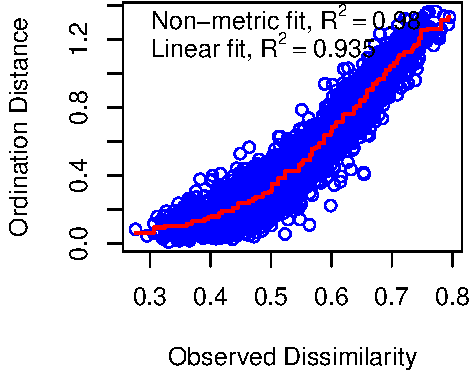
\includegraphics{Technical-supplement_files/figure-latex/fig-margin-1} \caption[Stressplot for NMDS - shows ordination distance vs dissimilarity (in Jaccard distance, in our case)]{Stressplot for NMDS - shows ordination distance vs dissimilarity (in Jaccard distance, in our case)}\label{fig:fig-margin}
\end{marginfigure}

We then use the \texttt{baselines} package
(\protect\hyperlink{ref-burge_2022_baselines}{Burge, 2022}) to calculate
the pre-human baseline. It also creates a spatial ellipse for the
baseline and a spatial points object. Note that the metadata (`metadf')
needs to have the same order as the data that went into the ordination!
This requirement also applies to most of the functions in \texttt{vegan}
too, by the way.

\begin{Shaded}
\begin{Highlighting}[]
\NormalTok{distsOut }\OtherTok{\textless{}{-}} \FunctionTok{calcEllipseDists}\NormalTok{(}\AttributeTok{metadf =}\NormalTok{ imps, }
                        \AttributeTok{ord =}\NormalTok{ okMeta,}
                        \AttributeTok{group =} \StringTok{"period"}\NormalTok{, }
                        \AttributeTok{reflev =} \StringTok{"Pre{-}Human"}\NormalTok{)}

\CommentTok{\# distsOut returns a list {-} what are the names}
\FunctionTok{names}\NormalTok{(distsOut)}
\end{Highlighting}
\end{Shaded}

\begin{verbatim}
## [1] "distDF"              "baseline_polygon"    "all_points"         
## [4] "baseline_polygon_DF"
\end{verbatim}

The \texttt{distDF} is the dataframe with the original metadata supplied
to the function, the NMDS scores for each point, the centroid for each
period, and the distance from ellipse and baseline for the selected
baseline level. This is what you will typically use. The
\texttt{baseline\_polygon} and \texttt{all\_points} are spatial objects
and can be used with base plotting methods, and other spatial functions.
\texttt{baseline\_polygon\_DF} is the baseline ellipse converted to a
dataframe for easier plotting with \texttt{ggplot2}
(\protect\hyperlink{ref-wickham_2016_ggplot2}{Wickham, 2016}).

\begin{Shaded}
\begin{Highlighting}[]
\NormalTok{metaScores }\OtherTok{\textless{}{-}}\NormalTok{ distsOut[[}\StringTok{"distDF"}\NormalTok{]] }\SpecialCharTok{\%\textgreater{}\%}
  \FunctionTok{mutate}\NormalTok{(}\AttributeTok{period =} \FunctionTok{as.factor}\NormalTok{(period))}

\FunctionTok{head}\NormalTok{(metaScores, }\DecValTok{2}\NormalTok{)}
\end{Highlighting}
\end{Shaded}

\begin{verbatim}
##        YEAR DEPTH       SITE    period      NMDS1       NMDS2  centroid1
## 1  84.83404   560 Rotonuiaha Pre-Human -0.4353609 -0.12586729 -0.2746514
## 2 129.42979   550 Rotonuiaha Pre-Human -0.4996545 -0.02659776 -0.2746514
##     centroid2 distEllipse disCentroid
## 1 -0.00574629           0   0.2006405
## 2 -0.00574629           0   0.2259671
\end{verbatim}

Here we extract the \texttt{baseline\_polygon\_DF} to a new standalone
object for more concise plotting code, and get the centroid scores for
the pre-human period.

\begin{Shaded}
\begin{Highlighting}[]
\NormalTok{baselineEllipse }\OtherTok{\textless{}{-}}\NormalTok{ distsOut[[}\StringTok{"baseline\_polygon\_DF"}\NormalTok{]]}

\CommentTok{\# get centroid for pre{-}human ellipse}

\NormalTok{centroidCoord }\OtherTok{\textless{}{-}}\NormalTok{ metaScores }\SpecialCharTok{\%\textgreater{}\%} 
  \FunctionTok{filter}\NormalTok{(period }\SpecialCharTok{==} \StringTok{"Pre{-}Human"}\NormalTok{) }\SpecialCharTok{\%\textgreater{}\%}
  \FunctionTok{slice}\NormalTok{(}\DecValTok{1}\NormalTok{) }\SpecialCharTok{\%\textgreater{}\%}
\NormalTok{  dplyr}\SpecialCharTok{::}\FunctionTok{select}\NormalTok{(SITE, centroid1, centroid2)}
\end{Highlighting}
\end{Shaded}

\hypertarget{plot-nmds-and-baseline-ellipse}{%
\subsection{Plot NMDS and baseline
ellipse}\label{plot-nmds-and-baseline-ellipse}}

We can now plot the results of the ordination. \texttt{coord\_equal()}
is required when plotting ordinations in \texttt{ggplot2}
(\protect\hyperlink{ref-wickham_2016_ggplot2}{Wickham, 2016}) - base
plot uses a 1:1 aspect ratio for the x and y axes automatically for
ordinations.

\begin{Shaded}
\begin{Highlighting}[]
\NormalTok{ptSize }\OtherTok{\textless{}{-}} \FloatTok{2.5}
\NormalTok{nmdsPlot }\OtherTok{\textless{}{-}} \FunctionTok{ggplot}\NormalTok{() }\SpecialCharTok{+} 
  \FunctionTok{coord\_equal}\NormalTok{() }\SpecialCharTok{+} 
  \FunctionTok{geom\_hline}\NormalTok{(}\AttributeTok{colour =} \StringTok{"grey"}\NormalTok{, }\AttributeTok{linetype =} \StringTok{"dashed"}\NormalTok{, }
             \AttributeTok{yintercept =} \DecValTok{0}\NormalTok{) }\SpecialCharTok{+}
  \FunctionTok{geom\_vline}\NormalTok{(}\AttributeTok{colour =} \StringTok{"grey"}\NormalTok{, }\AttributeTok{linetype =} \StringTok{"dashed"}\NormalTok{, }
             \AttributeTok{xintercept =} \DecValTok{0}\NormalTok{) }\SpecialCharTok{+}
  \FunctionTok{geom\_polygon}\NormalTok{(}\AttributeTok{data =}\NormalTok{ baselineEllipse, }
               \FunctionTok{aes}\NormalTok{(}\AttributeTok{x =}\NormalTok{ NMDS1, }\AttributeTok{y =}\NormalTok{ NMDS2,}
                   \AttributeTok{fill =}\NormalTok{ group),}
               \AttributeTok{alpha =} \FloatTok{0.5}\NormalTok{, }\AttributeTok{show.legend =} \ConstantTok{FALSE}\NormalTok{) }\SpecialCharTok{+}
  \FunctionTok{geom\_point}\NormalTok{(}\AttributeTok{data =}\NormalTok{ metaScores, }
             \FunctionTok{aes}\NormalTok{(}\AttributeTok{x =}\NormalTok{ NMDS1, }\AttributeTok{y =}\NormalTok{ NMDS2,}
                 \AttributeTok{fill =}\NormalTok{ period),}
             \AttributeTok{size =}\NormalTok{ ptSize, }\AttributeTok{colour =} \StringTok{"black"}\NormalTok{, }\AttributeTok{shape =} \DecValTok{21}\NormalTok{,}
             \AttributeTok{stroke =} \FloatTok{0.8}\NormalTok{) }\SpecialCharTok{+}
    \FunctionTok{geom\_text}\NormalTok{(}\AttributeTok{data =}\NormalTok{ centroidCoord, }
            \FunctionTok{aes}\NormalTok{(}\AttributeTok{x =}\NormalTok{ centroid1, }\AttributeTok{y =}\NormalTok{ centroid2), }
            \AttributeTok{label =} \StringTok{"X"}\NormalTok{,}
            \AttributeTok{colour =} \StringTok{"white"}\NormalTok{,}
            \AttributeTok{size =} \DecValTok{12}\NormalTok{) }\SpecialCharTok{+}
  \FunctionTok{scale\_fill\_brewer}\NormalTok{(}\StringTok{"Time period"}\NormalTok{, }
                    \AttributeTok{palette =} \StringTok{"YlGnBu"}\NormalTok{,}
                    \AttributeTok{direction =} \SpecialCharTok{{-}}\DecValTok{1}\NormalTok{,}
                    \AttributeTok{limits =} \FunctionTok{c}\NormalTok{(}\StringTok{"Pre{-}Human"}\NormalTok{, }
                               \StringTok{"Post{-}Polynesian"}\NormalTok{, }
                               \StringTok{"Post{-}European"}\NormalTok{),}
                    \AttributeTok{labels =} \FunctionTok{c}\NormalTok{(}\StringTok{"Pre{-}Human"}\NormalTok{, }
                               \StringTok{"Post{-}Polynesian"}\NormalTok{, }
                               \StringTok{"Post{-}European"}\NormalTok{)) }\SpecialCharTok{+}
  \FunctionTok{guides}\NormalTok{(}\AttributeTok{fill =} \FunctionTok{guide\_legend}\NormalTok{(}\AttributeTok{title.position =} \StringTok{"top"}\NormalTok{,}
                             \AttributeTok{title.hjust =} \FloatTok{0.5}\NormalTok{,}
                             \AttributeTok{nrow =} \DecValTok{2}\NormalTok{, }\AttributeTok{byrow =} \ConstantTok{TRUE}\NormalTok{))}\SpecialCharTok{+}
  \FunctionTok{theme\_bw}\NormalTok{() }\SpecialCharTok{+}
  \FunctionTok{labs}\NormalTok{(}\AttributeTok{tag =} \StringTok{"(a)"}\NormalTok{) }\SpecialCharTok{+}
  \FunctionTok{theme}\NormalTok{(}\AttributeTok{legend.position =} \StringTok{"bottom"}\NormalTok{, }
        \AttributeTok{panel.grid =} \FunctionTok{element\_blank}\NormalTok{(),}
        \AttributeTok{plot.tag.position =} \StringTok{"topleft"}\NormalTok{)}
\end{Highlighting}
\end{Shaded}

\hypertarget{plot-distance-methods-figure}{%
\subsection{Plot distance methods
figure}\label{plot-distance-methods-figure}}

We don't plot the nmds plot yet however; we also demonstrate the
distance between each point and the reference baseline. The function
\texttt{gDistance} (\texttt{rgeos} package) calculates the minimum
distance from each of our points to the polygon automatically. To
demonstrate, we convert the reference baseline polygon to points and
then select the polygon-point with the minimum distance to our sample
points and plot that. You will also need the \texttt{sp} package.

\begin{Shaded}
\begin{Highlighting}[]
\CommentTok{\# convert the polygon to points}
\NormalTok{baselinePoints }\OtherTok{\textless{}{-}} \FunctionTok{SpatialPoints}\NormalTok{(distsOut[[}
  \StringTok{"baseline\_polygon"}\NormalTok{]]}\SpecialCharTok{@}\NormalTok{polygons[[}
    \DecValTok{1}\NormalTok{]]}\SpecialCharTok{@}\NormalTok{Polygons[[}\DecValTok{1}\NormalTok{]]}\SpecialCharTok{@}\NormalTok{coords)}

\CommentTok{\# extract all the points that are not}
\CommentTok{\# pre{-}human}
\NormalTok{samplePoints }\OtherTok{\textless{}{-}}\NormalTok{ distsOut[[}
  \StringTok{"all\_points"}\NormalTok{]][distsOut[[}
    \StringTok{"all\_points"}\NormalTok{]]}\SpecialCharTok{$}\NormalTok{period }\SpecialCharTok{!=} \StringTok{"Pre{-}Human"}\NormalTok{, ]}

\CommentTok{\# calculate distance from each sample point }
\CommentTok{\# to each baseline point}
\NormalTok{dists }\OtherTok{\textless{}{-}} \FunctionTok{gDistance}\NormalTok{(samplePoints, baselinePoints, }
                   \AttributeTok{byid =} \ConstantTok{TRUE}\NormalTok{)}
 

\CommentTok{\# get the id of the closest point from the baseline}
\CommentTok{\# to each sample point}
\NormalTok{theMins }\OtherTok{\textless{}{-}} \FunctionTok{as.numeric}\NormalTok{(}
  \FunctionTok{sapply}\NormalTok{(}\AttributeTok{USE.NAMES =} \ConstantTok{FALSE}\NormalTok{, }
         \DecValTok{1}\SpecialCharTok{:}\FunctionTok{length}\NormalTok{(samplePoints),}
         \ControlFlowTok{function}\NormalTok{(x) }\FunctionTok{which.min}\NormalTok{(dists[, x])))}

\CommentTok{\# create a df for the arrows that go from each point}
\CommentTok{\# to the closest point of the ellipse}
\CommentTok{\# NB this is not required for your own analysis}
\NormalTok{segDF }\OtherTok{\textless{}{-}} \FunctionTok{do.call}\NormalTok{(}
  \StringTok{"rbind"}\NormalTok{, }
  \FunctionTok{lapply}\NormalTok{(}\DecValTok{1}\SpecialCharTok{:}\FunctionTok{length}\NormalTok{(samplePoints),}
         \ControlFlowTok{function}\NormalTok{(x)\{}
           \FunctionTok{data.frame}\NormalTok{(}
             \AttributeTok{x1 =}\NormalTok{ samplePoints}\SpecialCharTok{@}\NormalTok{coords[x,}\DecValTok{1}\NormalTok{], }
             \AttributeTok{y1 =}\NormalTok{ samplePoints}\SpecialCharTok{@}\NormalTok{coords[x,}\DecValTok{2}\NormalTok{], }
             \AttributeTok{x0 =} \FunctionTok{as.numeric}\NormalTok{(}
\NormalTok{               baselinePoints}\SpecialCharTok{@}\NormalTok{coords[theMins[x], }\DecValTok{1}\NormalTok{]), }
             \AttributeTok{y0 =} \FunctionTok{as.numeric}\NormalTok{(}
\NormalTok{               baselinePoints}\SpecialCharTok{@}\NormalTok{coords[theMins[x], }\DecValTok{2}\NormalTok{]))}
\NormalTok{         \}) }
\NormalTok{)}


\CommentTok{\# plot the distance methods plot}
\NormalTok{distancePlot }\OtherTok{\textless{}{-}} \FunctionTok{ggplot}\NormalTok{() }\SpecialCharTok{+} 
  \FunctionTok{geom\_point}\NormalTok{(}\AttributeTok{data =} \FunctionTok{as.data.frame}\NormalTok{(baselinePoints),}
             \FunctionTok{aes}\NormalTok{(}\AttributeTok{x =}\NormalTok{ coords.x1, }\AttributeTok{y =}\NormalTok{ coords.x2),}
             \AttributeTok{shape =} \DecValTok{1}\NormalTok{) }\SpecialCharTok{+}
  \FunctionTok{geom\_point}\NormalTok{(}\AttributeTok{data =} \FunctionTok{as.data.frame}\NormalTok{(samplePoints),}
             \FunctionTok{aes}\NormalTok{(}\AttributeTok{x =}\NormalTok{ NMDS1, }\AttributeTok{y =}\NormalTok{ NMDS2,}
                 \AttributeTok{shape =}\NormalTok{ period),}
             \AttributeTok{size =}\NormalTok{ ptSize) }\SpecialCharTok{+}
  \FunctionTok{geom\_hline}\NormalTok{(}\AttributeTok{colour =} \StringTok{"grey"}\NormalTok{, }\AttributeTok{linetype =} \StringTok{"dashed"}\NormalTok{, }
             \AttributeTok{yintercept =} \DecValTok{0}\NormalTok{) }\SpecialCharTok{+}
  \FunctionTok{geom\_vline}\NormalTok{(}\AttributeTok{colour =} \StringTok{"grey"}\NormalTok{, }\AttributeTok{linetype =} \StringTok{"dashed"}\NormalTok{, }
             \AttributeTok{xintercept =} \DecValTok{0}\NormalTok{) }\SpecialCharTok{+}
  \FunctionTok{geom\_segment}\NormalTok{(}\AttributeTok{data =}\NormalTok{ segDF,}
               \AttributeTok{colour =} \StringTok{"grey"}\NormalTok{,}
               \FunctionTok{aes}\NormalTok{(}\AttributeTok{x =}\NormalTok{ x0, }\AttributeTok{y =}\NormalTok{ y0,}
                   \AttributeTok{xend =}\NormalTok{ x1, }\AttributeTok{yend =}\NormalTok{ y1),}
               \AttributeTok{arrow =} \FunctionTok{arrow}\NormalTok{(}\AttributeTok{length =} \FunctionTok{unit}\NormalTok{(}\FloatTok{0.1}\NormalTok{, }\StringTok{"inches"}\NormalTok{),}
                             \AttributeTok{angle =} \DecValTok{20}\NormalTok{)) }\SpecialCharTok{+}
    \FunctionTok{scale\_shape\_manual}\NormalTok{(}\StringTok{"Time period"}\NormalTok{, }
                       \AttributeTok{values =} \FunctionTok{c}\NormalTok{(}\DecValTok{16}\NormalTok{, }\DecValTok{17}\NormalTok{),}
                    \AttributeTok{limits =} \FunctionTok{c}\NormalTok{(}\StringTok{"Post{-}Polynesian"}\NormalTok{, }
                               \StringTok{"Post{-}European"}\NormalTok{),}
                    \AttributeTok{labels =} \FunctionTok{c}\NormalTok{(}\StringTok{"Post{-}Polynesian"}\NormalTok{, }
                               \StringTok{"Post{-}European"}\NormalTok{)) }\SpecialCharTok{+}
  \FunctionTok{coord\_equal}\NormalTok{() }\SpecialCharTok{+}
  \FunctionTok{theme\_bw}\NormalTok{() }\SpecialCharTok{+}
  \FunctionTok{guides}\NormalTok{(}\AttributeTok{shape =} \FunctionTok{guide\_legend}\NormalTok{(}\AttributeTok{title.position =} \StringTok{"top"}\NormalTok{,}
                              \AttributeTok{title.hjust =} \FloatTok{0.5}\NormalTok{,}
                              \AttributeTok{nrow =} \DecValTok{2}\NormalTok{))}\SpecialCharTok{+}
  \FunctionTok{labs}\NormalTok{(}\AttributeTok{tag =} \StringTok{"(b)"}\NormalTok{, }\AttributeTok{x =} \StringTok{"NMDS1"}\NormalTok{, }\AttributeTok{y =} \StringTok{"NMDS2"}\NormalTok{) }\SpecialCharTok{+}
  \FunctionTok{theme}\NormalTok{(}\AttributeTok{legend.position =} \StringTok{"bottom"}\NormalTok{, }
        \AttributeTok{panel.grid =} \FunctionTok{element\_blank}\NormalTok{(),}
        \AttributeTok{plot.tag.position =} \StringTok{"topleft"}\NormalTok{)}


\CommentTok{\# we use package egg to put the plots together. }
\CommentTok{\# Others are fine too.}
\NormalTok{egg}\SpecialCharTok{::}\FunctionTok{ggarrange}\NormalTok{(nmdsPlot, distancePlot, }\AttributeTok{nrow =} \DecValTok{1}\NormalTok{,}
               \AttributeTok{labels =} \FunctionTok{c}\NormalTok{(}\StringTok{"a"}\NormalTok{, }\StringTok{"b"}\NormalTok{),}
               \AttributeTok{label.args =} \FunctionTok{list}\NormalTok{(}\AttributeTok{gp =}\NormalTok{ grid}\SpecialCharTok{::}\FunctionTok{gpar}\NormalTok{(}
                 \AttributeTok{font =} \DecValTok{2}\NormalTok{,}
                 \AttributeTok{cex =} \FloatTok{1.2}\NormalTok{)))}
\end{Highlighting}
\end{Shaded}

\begin{figure*}
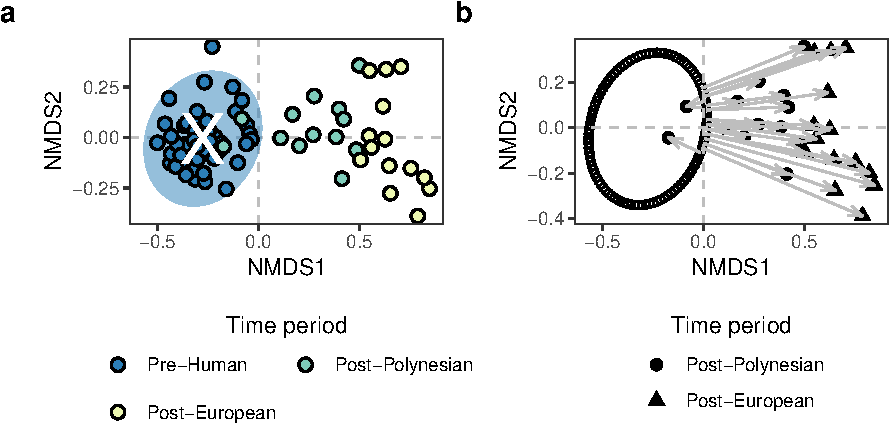
\includegraphics{Technical-supplement_files/figure-latex/unnamed-chunk-3-1} \caption[NMDS showing pre-human baselines of a 95\% CI ellipse (blue polygon) and the centroid (white X) (a)]{NMDS showing pre-human baselines of a 95\% CI ellipse (blue polygon) and the centroid (white X) (a); and distance from both baselines (b). NB points within the polygon get a distance of zero}\label{fig:unnamed-chunk-3}
\end{figure*}

\clearpage

\hypertarget{distance-from-baseline-over-time-statistical-model}{%
\subsection{Distance from baseline over time: statistical
model}\label{distance-from-baseline-over-time-statistical-model}}

Here we run a linear model, checking whether the post-Polynesian or
post-European period distance from baseline differs to zero, and whether
it changes over time. Read the paper
(\protect\hyperlink{ref-wilmshurst_96_forest}{Wilmshurst \& McGlone,
1996}) to see why that might be!

\begin{Shaded}
\begin{Highlighting}[]
\NormalTok{excludingPreHuman }\OtherTok{\textless{}{-}}\NormalTok{ metaScores[}
\NormalTok{  metaScores}\SpecialCharTok{$}\NormalTok{period }\SpecialCharTok{!=} \StringTok{"Pre{-}Human"}\NormalTok{, ]}

\NormalTok{lmModEllipse }\OtherTok{\textless{}{-}} \FunctionTok{lm}\NormalTok{(}\AttributeTok{data =}\NormalTok{ excludingPreHuman, }
   \AttributeTok{formula =}\NormalTok{ distEllipse }\SpecialCharTok{\textasciitilde{}}\NormalTok{ YEAR }\SpecialCharTok{*}\NormalTok{ period,}
   \AttributeTok{na.action =} \StringTok{"na.fail"}\NormalTok{)}
\end{Highlighting}
\end{Shaded}

\begin{Shaded}
\begin{Highlighting}[]
\NormalTok{modComp }\OtherTok{\textless{}{-}} \FunctionTok{dredge}\NormalTok{(lmModEllipse)}

\NormalTok{knitr}\SpecialCharTok{::}\FunctionTok{kable}\NormalTok{(modComp }\SpecialCharTok{\%\textgreater{}\%} 
               \FunctionTok{as.data.frame}\NormalTok{() }\SpecialCharTok{\%\textgreater{}\%}
               \FunctionTok{mutate}\NormalTok{(}\FunctionTok{across}\NormalTok{(}\FunctionTok{where}\NormalTok{(is.numeric), }
\NormalTok{                         \textbackslash{}(x) }\FunctionTok{sprintf}\NormalTok{(x, }
                         \AttributeTok{fmt =} \StringTok{"\%.3f"}\NormalTok{))) }\SpecialCharTok{\%\textgreater{}\%}
               \FunctionTok{rename}\NormalTok{(}\AttributeTok{Intercept =} \StringTok{\textasciigrave{}}\AttributeTok{(Intercept)}\StringTok{\textasciigrave{}}\NormalTok{), }
             \AttributeTok{caption =} \StringTok{"Model comparison table for distance from baseline over time. The year column is the coefficient estimate for year."}\NormalTok{)}
\end{Highlighting}
\end{Shaded}

\begin{longtable}[]{@{}
  >{\raggedright\arraybackslash}p{(\columnwidth - 18\tabcolsep) * \real{0.0411}}
  >{\raggedright\arraybackslash}p{(\columnwidth - 18\tabcolsep) * \real{0.1370}}
  >{\raggedright\arraybackslash}p{(\columnwidth - 18\tabcolsep) * \real{0.0959}}
  >{\raggedright\arraybackslash}p{(\columnwidth - 18\tabcolsep) * \real{0.0822}}
  >{\raggedright\arraybackslash}p{(\columnwidth - 18\tabcolsep) * \real{0.1644}}
  >{\raggedright\arraybackslash}p{(\columnwidth - 18\tabcolsep) * \real{0.0822}}
  >{\raggedright\arraybackslash}p{(\columnwidth - 18\tabcolsep) * \real{0.0959}}
  >{\raggedright\arraybackslash}p{(\columnwidth - 18\tabcolsep) * \real{0.1096}}
  >{\raggedright\arraybackslash}p{(\columnwidth - 18\tabcolsep) * \real{0.0959}}
  >{\raggedright\arraybackslash}p{(\columnwidth - 18\tabcolsep) * \real{0.0959}}@{}}
\caption{Model comparison table for distance from baseline over time.
The year column is the coefficient estimate for year.}\tabularnewline
\toprule\noalign{}
\begin{minipage}[b]{\linewidth}\raggedright
\end{minipage} & \begin{minipage}[b]{\linewidth}\raggedright
Intercept
\end{minipage} & \begin{minipage}[b]{\linewidth}\raggedright
period
\end{minipage} & \begin{minipage}[b]{\linewidth}\raggedright
YEAR
\end{minipage} & \begin{minipage}[b]{\linewidth}\raggedright
period:YEAR
\end{minipage} & \begin{minipage}[b]{\linewidth}\raggedright
df
\end{minipage} & \begin{minipage}[b]{\linewidth}\raggedright
logLik
\end{minipage} & \begin{minipage}[b]{\linewidth}\raggedright
AICc
\end{minipage} & \begin{minipage}[b]{\linewidth}\raggedright
delta
\end{minipage} & \begin{minipage}[b]{\linewidth}\raggedright
weight
\end{minipage} \\
\midrule\noalign{}
\endfirsthead
\toprule\noalign{}
\begin{minipage}[b]{\linewidth}\raggedright
\end{minipage} & \begin{minipage}[b]{\linewidth}\raggedright
Intercept
\end{minipage} & \begin{minipage}[b]{\linewidth}\raggedright
period
\end{minipage} & \begin{minipage}[b]{\linewidth}\raggedright
YEAR
\end{minipage} & \begin{minipage}[b]{\linewidth}\raggedright
period:YEAR
\end{minipage} & \begin{minipage}[b]{\linewidth}\raggedright
df
\end{minipage} & \begin{minipage}[b]{\linewidth}\raggedright
logLik
\end{minipage} & \begin{minipage}[b]{\linewidth}\raggedright
AICc
\end{minipage} & \begin{minipage}[b]{\linewidth}\raggedright
delta
\end{minipage} & \begin{minipage}[b]{\linewidth}\raggedright
weight
\end{minipage} \\
\midrule\noalign{}
\endhead
\bottomrule\noalign{}
\endlastfoot
3 & -1.268 & NA & 0.001 & NA & 3.000 & 25.969 & -44.894 & 0.000 &
0.548 \\
8 & -3.416 & + & 0.002 & + & 5.000 & 28.209 & -43.562 & 1.333 & 0.281 \\
4 & -1.103 & + & 0.001 & NA & 4.000 & 26.194 & -42.570 & 2.324 &
0.171 \\
2 & 0.670 & + & NA & NA & 3.000 & 13.918 & -20.793 & 24.101 & 0.000 \\
1 & 0.480 & NA & NA & NA & 2.000 & -0.293 & 5.085 & 49.980 & 0.000 \\
\end{longtable}

\begin{Shaded}
\begin{Highlighting}[]
\CommentTok{\# preferred model}
\NormalTok{simpleLM }\OtherTok{\textless{}{-}} \FunctionTok{lm}\NormalTok{(}\AttributeTok{data =}\NormalTok{ excludingPreHuman, }
   \AttributeTok{formula =}\NormalTok{ distEllipse }\SpecialCharTok{\textasciitilde{}}\NormalTok{ YEAR)}
\end{Highlighting}
\end{Shaded}

The diagnostic plots from the model look pretty good (Fig.
\ref{fig:lmModDiag}; just one of several plots shown).

\begin{Shaded}
\begin{Highlighting}[]
\FunctionTok{plot}\NormalTok{(lmModEllipse, }\AttributeTok{which =} \DecValTok{1}\NormalTok{)}
\end{Highlighting}
\end{Shaded}

\begin{marginfigure}
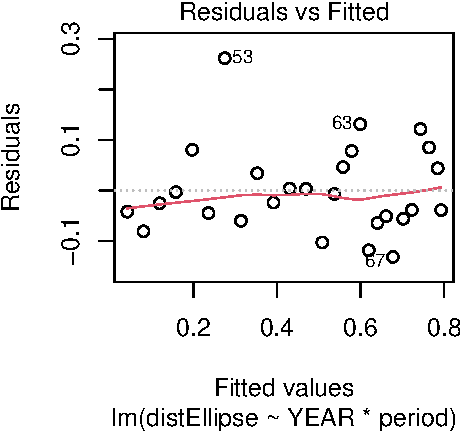
\includegraphics{Technical-supplement_files/figure-latex/lmModDiag-1} \caption[Diagnostic plot from linear model]{Diagnostic plot from linear model}\label{fig:lmModDiag}
\end{marginfigure}

We inspect the residuals of the linear model for temporal
autocorrelation (Fig. \ref{fig:firstacf}). These look ok (you don't
consider lag = 0!), so we won't go on to fit a model with
autocorrelation. We demonstrate how to compare models with lag 1 and lag
2 autocorrelations using the \texttt{gls} function from package
\texttt{nlme}

\begin{Shaded}
\begin{Highlighting}[]
\FunctionTok{acf}\NormalTok{(}\FunctionTok{resid}\NormalTok{(simpleLM), }\AttributeTok{main =} \StringTok{""}\NormalTok{)}
\end{Highlighting}
\end{Shaded}

\begin{marginfigure}
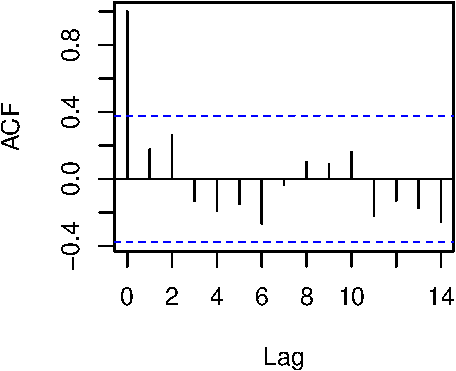
\includegraphics{Technical-supplement_files/figure-latex/firstacf-1} \caption[Checking for temporal autocorrelation in model residuals]{Checking for temporal autocorrelation in model residuals}\label{fig:firstacf}
\end{marginfigure}

\hypertarget{demonstration-of-a-gls-model}{%
\subsection{Demonstration of a gls
model}\label{demonstration-of-a-gls-model}}

In this case, had we used a gls model, it would have been slightly more
conservative in terms of \emph{T} values but no drastic changes. We show
a gls model with lag 1 and lag 2 temporal autocorrelation, and a `null'
model of no temporal autocorrelation - but all have the same fixed
effect of year. As the fixed effects are the same we compare using REML
(if they differed, ML would be a better choice see discussion
\href{https://stats.stackexchange.com/questions/16013/allowed-comparisons-of-mixed-effects-models-random-effects-primarily/16015\#16015}{here}).

\begin{Shaded}
\begin{Highlighting}[]
\CommentTok{\# model with lag 1 correlation}
\NormalTok{simpleGLS }\OtherTok{\textless{}{-}} \FunctionTok{gls}\NormalTok{(distEllipse }\SpecialCharTok{\textasciitilde{}}\NormalTok{ YEAR,}
                           \AttributeTok{data =}\NormalTok{ excludingPreHuman,}
                 \AttributeTok{correlation =} \FunctionTok{corARMA}\NormalTok{(}\AttributeTok{p =} \DecValTok{1}\NormalTok{),}
                  \AttributeTok{method =} \StringTok{"REML"}\NormalTok{,}
                 \AttributeTok{na.action =} \StringTok{"na.fail"}\NormalTok{)}


\CommentTok{\# same model but with lag 2 correlation}
\NormalTok{simpleGLS2 }\OtherTok{\textless{}{-}} \FunctionTok{update}\NormalTok{(simpleGLS, }
                     \AttributeTok{correlation =} \FunctionTok{corARMA}\NormalTok{(}\AttributeTok{p =} \DecValTok{2}\NormalTok{))}

\CommentTok{\# same model but with no temporal autocorrelation}
\NormalTok{simpleGLS0 }\OtherTok{\textless{}{-}} \FunctionTok{update}\NormalTok{(simpleGLS, }
                     \AttributeTok{correlation =} \ConstantTok{NULL}\NormalTok{)}

\CommentTok{\# compare models}
\FunctionTok{anova}\NormalTok{(simpleGLS, simpleGLS2)}
\end{Highlighting}
\end{Shaded}

\begin{verbatim}
##            Model df       AIC       BIC   logLik   Test  L.Ratio p-value
## simpleGLS      1  4 -22.35919 -17.48369 15.17960                        
## simpleGLS2     2  5 -23.06715 -16.97277 16.53357 1 vs 2 2.707956  0.0998
\end{verbatim}

\begin{Shaded}
\begin{Highlighting}[]
\FunctionTok{anova}\NormalTok{(simpleGLS, simpleGLS2)}
\end{Highlighting}
\end{Shaded}

\begin{verbatim}
##            Model df       AIC       BIC   logLik   Test  L.Ratio p-value
## simpleGLS      1  4 -22.35919 -17.48369 15.17960                        
## simpleGLS2     2  5 -23.06715 -16.97277 16.53357 1 vs 2 2.707956  0.0998
\end{verbatim}

\begin{Shaded}
\begin{Highlighting}[]
\CommentTok{\# combine model summaries into dataframes}
\CommentTok{\# to print as a table}
\NormalTok{glsSummary }\OtherTok{\textless{}{-}} \FunctionTok{data.frame}\NormalTok{(}\AttributeTok{Model =} \StringTok{"gls"}\NormalTok{,}
                         \FunctionTok{summary}\NormalTok{(simpleGLS)}\SpecialCharTok{$}\NormalTok{tTable) }\SpecialCharTok{\%\textgreater{}\%}
  \FunctionTok{rownames\_to\_column}\NormalTok{(}\StringTok{"Parameter"}\NormalTok{) }\SpecialCharTok{\%\textgreater{}\%}
  \FunctionTok{rename}\NormalTok{(}\AttributeTok{Estimate =}\NormalTok{ Value)}

\NormalTok{lmSummary }\OtherTok{\textless{}{-}} \FunctionTok{data.frame}\NormalTok{(}\AttributeTok{Model =} \StringTok{"lm"}\NormalTok{, }
                        \FunctionTok{summary}\NormalTok{(simpleLM)}\SpecialCharTok{$}\NormalTok{coefficient) }\SpecialCharTok{\%\textgreater{}\%}
  \FunctionTok{rownames\_to\_column}\NormalTok{(}\StringTok{"Parameter"}\NormalTok{) }\SpecialCharTok{\%\textgreater{}\%}
  \FunctionTok{rename}\NormalTok{(}\AttributeTok{p.value =}\NormalTok{ Pr...t..,}
       \AttributeTok{Std.Error =}\NormalTok{ Std..Error)}

\NormalTok{knitr}\SpecialCharTok{::}\FunctionTok{kable}\NormalTok{(}\FunctionTok{bind\_rows}\NormalTok{(glsSummary, lmSummary) }\SpecialCharTok{\%\textgreater{}\%}
               \FunctionTok{mutate}\NormalTok{(}\AttributeTok{p.value =} \FunctionTok{sprintf}\NormalTok{(p.value, }\AttributeTok{fmt =} \StringTok{"\%.3f"}\NormalTok{)),}
                     \AttributeTok{digits =} \DecValTok{3}\NormalTok{,}
             \AttributeTok{caption =} \StringTok{"GLS and LM model summaries"}\NormalTok{)}
\end{Highlighting}
\end{Shaded}

\begin{longtable}[]{@{}llrrrl@{}}
\caption{GLS and LM model summaries}\tabularnewline
\toprule\noalign{}
Parameter & Model & Estimate & Std.Error & t.value & p.value \\
\midrule\noalign{}
\endfirsthead
\toprule\noalign{}
Parameter & Model & Estimate & Std.Error & t.value & p.value \\
\midrule\noalign{}
\endhead
\bottomrule\noalign{}
\endlastfoot
(Intercept) & gls & -1.272 & 0.185 & -6.880 & 0.000 \\
YEAR & gls & 0.001 & 0.000 & 9.546 & 0.000 \\
(Intercept) & lm & -1.268 & 0.144 & -8.808 & 0.000 \\
YEAR & lm & 0.001 & 0.000 & 12.243 & 0.000 \\
\end{longtable}

\hypertarget{interpretation-of-distance-from-baseline-model}{%
\subsection{Interpretation of distance-from-baseline
model}\label{interpretation-of-distance-from-baseline-model}}

For Rotonuiaha, we see that the intercept differs significantly to zero,
which, where we have a continuous predictor only, can be interpreted as
the model estimate when the continuous predictor (year) is set to zero.
This is not particularly meaningful in our case. However, the year
estimate means that for every 1 unit increase in year (i.e.~1 year),
there is a 0.001 increase in ecological (ordination) distance from
baseline, thus we see that distance from baseline is increasing from
time. We see the fitted relationship and raw data in Fig.
\ref{fig:predictinglm}. Code to make Fig. \ref{fig:predictinglm} is set
out below.

\begin{Shaded}
\begin{Highlighting}[]
\NormalTok{newYears }\OtherTok{\textless{}{-}} \FunctionTok{data.frame}\NormalTok{(}
  \AttributeTok{YEAR =} \FunctionTok{seq}\NormalTok{(}\AttributeTok{from =} \FunctionTok{min}\NormalTok{(excludingPreHuman}\SpecialCharTok{$}\NormalTok{YEAR), }
             \AttributeTok{to =} \FunctionTok{max}\NormalTok{(excludingPreHuman}\SpecialCharTok{$}\NormalTok{YEAR),}
             \AttributeTok{by =} \DecValTok{1}\NormalTok{)}
\NormalTok{  )}

\NormalTok{modelPreds }\OtherTok{\textless{}{-}} \FunctionTok{predict}\NormalTok{(simpleLM, }\AttributeTok{newdata =}\NormalTok{ newYears, }
                      \AttributeTok{interval =} \StringTok{"confidence"}\NormalTok{,}
                      \AttributeTok{level =} \FloatTok{0.95}\NormalTok{,}
                      \AttributeTok{se.fit =} \ConstantTok{TRUE}\NormalTok{)}
\NormalTok{newYears }\OtherTok{\textless{}{-}} \FunctionTok{data.frame}\NormalTok{(newYears, modelPreds[[}\DecValTok{1}\NormalTok{]])}

\FunctionTok{ggplot}\NormalTok{(newYears, }\FunctionTok{aes}\NormalTok{(}\AttributeTok{x =}\NormalTok{ YEAR, }\AttributeTok{y =}\NormalTok{ fit)) }\SpecialCharTok{+}
    \FunctionTok{geom\_point}\NormalTok{(}\AttributeTok{data =}\NormalTok{ excludingPreHuman, }
               \FunctionTok{aes}\NormalTok{(}\AttributeTok{y =}\NormalTok{ distEllipse),}
             \AttributeTok{shape =} \DecValTok{1}\NormalTok{) }\SpecialCharTok{+}
  \FunctionTok{geom\_ribbon}\NormalTok{(}\FunctionTok{aes}\NormalTok{(}\AttributeTok{ymin =}\NormalTok{ lwr, }\AttributeTok{ymax =}\NormalTok{ upr),}
              \AttributeTok{fill =} \FunctionTok{adjustcolor}\NormalTok{(}\StringTok{"grey50"}\NormalTok{, }\FloatTok{0.4}\NormalTok{), }
              \AttributeTok{linetype =} \StringTok{"dashed"}\NormalTok{) }\SpecialCharTok{+}
  \FunctionTok{geom\_line}\NormalTok{() }\SpecialCharTok{+}
  \FunctionTok{theme\_classic}\NormalTok{() }\SpecialCharTok{+} 
  \FunctionTok{labs}\NormalTok{(}\AttributeTok{x =} \StringTok{"Year"}\NormalTok{, }
       \AttributeTok{y =} \StringTok{"Distance from baseline in ordination space"}\NormalTok{)}
\end{Highlighting}
\end{Shaded}

\begin{marginfigure}
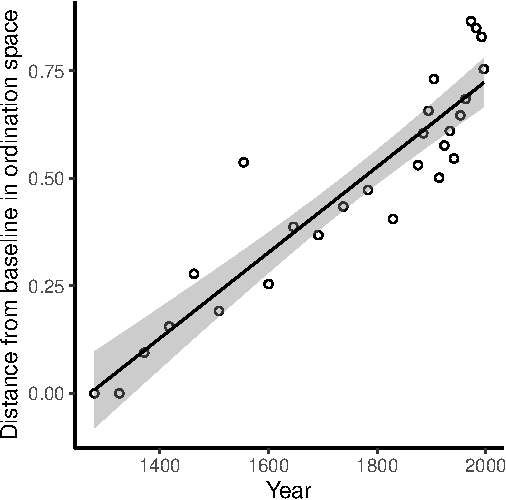
\includegraphics{Technical-supplement_files/figure-latex/predictinglm-1} \caption[Predictions from linear model]{Predictions from linear model}\label{fig:predictinglm}
\end{marginfigure}

\hypertarget{calculating-distance-from-baseline-ellipse-bayesian}{%
\section{Calculating distance from baseline (ellipse;
Bayesian)}\label{calculating-distance-from-baseline-ellipse-bayesian}}

We set out the code rather more briefly for calculating the ordination
distance from reference baseline (i.e.~an ellipse) for a Bayesian
analysis using the \texttt{boral} package
(\protect\hyperlink{ref-hui16_boral}{Hui, 2016}). The only differences
are in the calculation of the ellipse (code in \texttt{baselines}
package Burge (\protect\hyperlink{ref-burge_2022_baselines}{2022})) and
in the ordination itself.

Here we use a negative binomial family (poisson also possible, among
others) and allow for 2 dimensions with the argument
\texttt{lv.control\ =\ list(num.lv\ =\ 2)}, and a random effect for each
row (plot).

The diagnostic plots can be examined to check for fit - ideally there is
no `funnel' effect in the residuals. See Fig \ref{fig:boralModPlot}
(poisson) and Fig \ref{fig:boralModPlot2} (negative binomial) below.

\begin{Shaded}
\begin{Highlighting}[]
\CommentTok{\# this is not run in an interactive session, }
\CommentTok{\# as it takes a long time. }
\CommentTok{\# If the rdata objects (below) are not in }
\CommentTok{\# your working directory}
\CommentTok{\# you will need to run this code. }
\ControlFlowTok{if}\NormalTok{(}\SpecialCharTok{!}\FunctionTok{interactive}\NormalTok{())\{}
\NormalTok{  boralMod  }\OtherTok{\textless{}{-}} \FunctionTok{boral}\NormalTok{(}\AttributeTok{y =}\NormalTok{ rotonuiaha[}\SpecialCharTok{!}\NormalTok{metaCols], }
                     \AttributeTok{family =} \StringTok{"negative.binomial"}\NormalTok{, }
                     \AttributeTok{lv.control =} \FunctionTok{list}\NormalTok{(}\AttributeTok{num.lv =} \DecValTok{2}\NormalTok{),}
                     \AttributeTok{mcmc.control =} \FunctionTok{list}\NormalTok{(}\AttributeTok{seed =} \DecValTok{888}\NormalTok{),}
                     \AttributeTok{row.eff =} \StringTok{"fixed"}\NormalTok{,}
                     \AttributeTok{save.model =} \ConstantTok{FALSE}\NormalTok{, }
                     \AttributeTok{calc.ics =} \ConstantTok{FALSE}\NormalTok{)}
  
\NormalTok{  boralMod2  }\OtherTok{\textless{}{-}} \FunctionTok{boral}\NormalTok{(}\AttributeTok{y =}\NormalTok{ rotonuiaha[}\SpecialCharTok{!}\NormalTok{metaCols], }
                      \AttributeTok{family =} \StringTok{"poisson"}\NormalTok{, }
                      \AttributeTok{lv.control =} \FunctionTok{list}\NormalTok{(}\AttributeTok{num.lv =} \DecValTok{2}\NormalTok{),}
                      \AttributeTok{mcmc.control =} \FunctionTok{list}\NormalTok{(}\AttributeTok{seed =} \DecValTok{888}\NormalTok{),}
                      \AttributeTok{row.eff =} \StringTok{"fixed"}\NormalTok{,}
                      \AttributeTok{save.model =} \ConstantTok{FALSE}\NormalTok{, }
                      \AttributeTok{calc.ics =} \ConstantTok{FALSE}\NormalTok{)}
  
  \FunctionTok{save}\NormalTok{(boralMod, }\AttributeTok{file =} \StringTok{"boralMod1.Rda"}\NormalTok{)}
  \FunctionTok{save}\NormalTok{(boralMod2, }\AttributeTok{file =} \StringTok{"boralMod2.Rda"}\NormalTok{)}

\NormalTok{\}}
\end{Highlighting}
\end{Shaded}

\begin{Shaded}
\begin{Highlighting}[]
\ControlFlowTok{if}\NormalTok{(}\FunctionTok{interactive}\NormalTok{())\{}
  \FunctionTok{load}\NormalTok{(}\StringTok{"boralMod1.Rda"}\NormalTok{)}
  \FunctionTok{load}\NormalTok{(}\StringTok{"boralMod2.Rda"}\NormalTok{)}
\NormalTok{\} }
\end{Highlighting}
\end{Shaded}

\begin{Shaded}
\begin{Highlighting}[]
\FunctionTok{par}\NormalTok{(}\AttributeTok{mfrow =} \FunctionTok{c}\NormalTok{(}\DecValTok{2}\NormalTok{,}\DecValTok{2}\NormalTok{))}

\FunctionTok{plot}\NormalTok{(boralMod2)}
\end{Highlighting}
\end{Shaded}

\begin{figure}
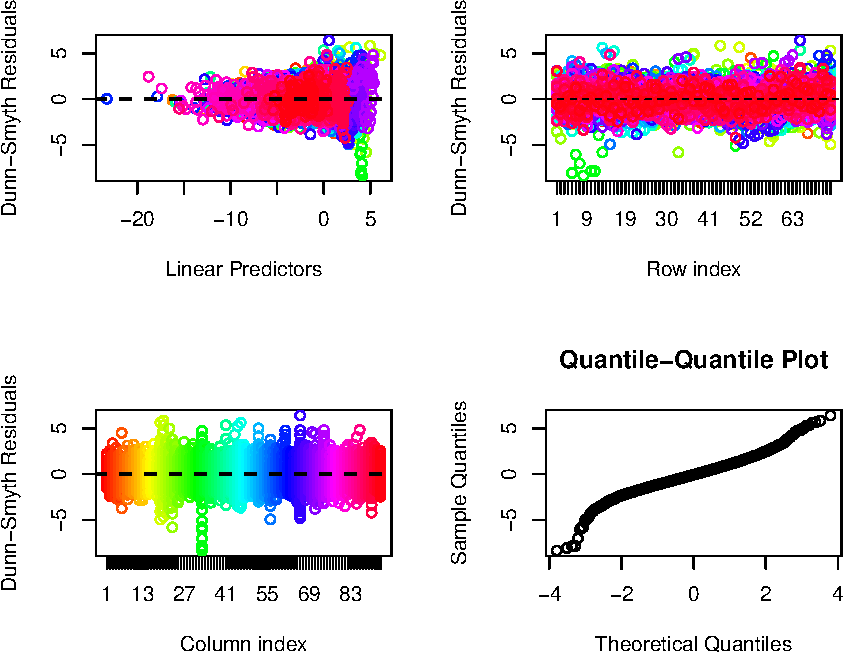
\includegraphics{Technical-supplement_files/figure-latex/boralModPlot-1} \caption[Boral model with poisson error structure]{Boral model with poisson error structure}\label{fig:boralModPlot}
\end{figure}

\begin{Shaded}
\begin{Highlighting}[]
\FunctionTok{par}\NormalTok{(}\AttributeTok{mfrow =} \FunctionTok{c}\NormalTok{(}\DecValTok{2}\NormalTok{,}\DecValTok{2}\NormalTok{))}

\FunctionTok{plot}\NormalTok{(boralMod)}
\end{Highlighting}
\end{Shaded}

\begin{figure}
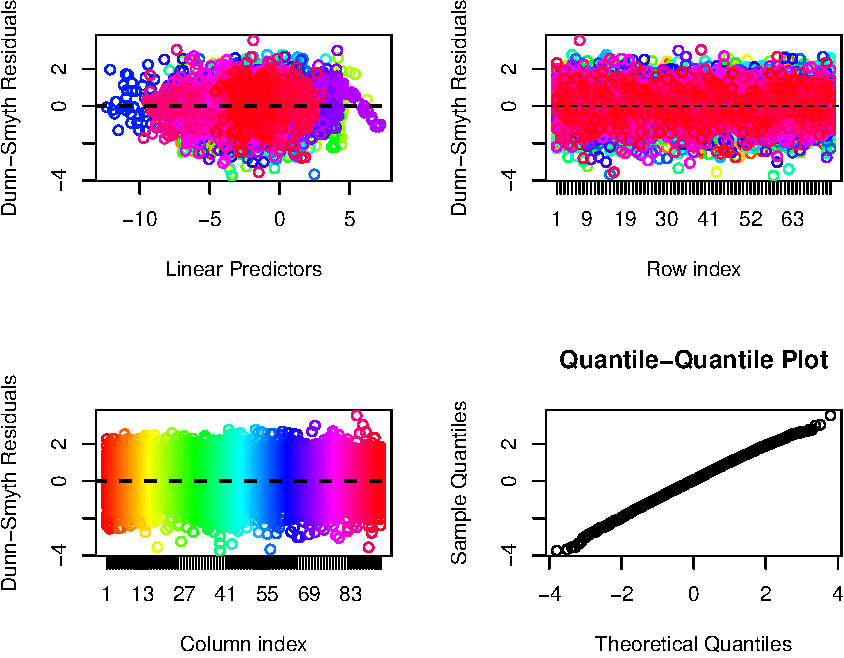
\includegraphics{Technical-supplement_files/figure-latex/boralModPlot2-1} \caption[Boral model with negative binomial error structure]{Boral model with negative binomial error structure}\label{fig:boralModPlot2}
\end{figure}

\begin{Shaded}
\begin{Highlighting}[]
\FunctionTok{par}\NormalTok{(}\AttributeTok{mfrow =} \FunctionTok{c}\NormalTok{(}\DecValTok{1}\NormalTok{,}\DecValTok{1}\NormalTok{))}
\end{Highlighting}
\end{Shaded}

We will use the negative binomial which looks better in terms of the
diagnostic plots (note the `funnel' effect with the poisson model
\ref{fig:boralModPlot}). Note that we set the random seed within the
function. If you amend this, there will be slight differences in the
positioning of the points.

\hypertarget{distance-from-baseline}{%
\subsection{Distance from baseline}\label{distance-from-baseline}}

We can calculate distance from baseline in a similar way to that with an
NMDS ordination (see Fig. \ref{fig:boralDistPlot}).

\begin{Shaded}
\begin{Highlighting}[]
\CommentTok{\# get distances}
\NormalTok{boralDists }\OtherTok{\textless{}{-}} \FunctionTok{calcEllipseDists}\NormalTok{(}\AttributeTok{metadf =}\NormalTok{ imps,}
                               \AttributeTok{ord =}\NormalTok{ boralMod,}
                               \AttributeTok{group =} \StringTok{"period"}\NormalTok{,}
                               \AttributeTok{reflev =} \StringTok{"Pre{-}Human"}\NormalTok{)}

\CommentTok{\# extract scores}
\NormalTok{boralDistDF }\OtherTok{\textless{}{-}}\NormalTok{ boralDists[[}\StringTok{"distDF"}\NormalTok{]]}
\NormalTok{boralRefPolygon }\OtherTok{\textless{}{-}}\NormalTok{ boralDists[[}\StringTok{"baseline\_polygon\_DF"}\NormalTok{]]}

\CommentTok{\# make plot}
\NormalTok{boralOrdPlot }\OtherTok{\textless{}{-}} \FunctionTok{ggplot}\NormalTok{(boralDistDF, }
                       \FunctionTok{aes}\NormalTok{(}\AttributeTok{x =}\NormalTok{ lvs1, }\AttributeTok{y =}\NormalTok{ lvs2)) }\SpecialCharTok{+}
  \FunctionTok{coord\_equal}\NormalTok{() }\SpecialCharTok{+}
  \FunctionTok{geom\_polygon}\NormalTok{(}\AttributeTok{data =}\NormalTok{ boralRefPolygon, }
               \FunctionTok{aes}\NormalTok{(}\AttributeTok{group =}\NormalTok{ group),}
               \AttributeTok{fill =} \FunctionTok{adjustcolor}\NormalTok{(}\StringTok{"grey"}\NormalTok{, }\FloatTok{0.5}\NormalTok{)) }\SpecialCharTok{+}
  \FunctionTok{geom\_point}\NormalTok{(}\FunctionTok{aes}\NormalTok{(}\AttributeTok{fill =}\NormalTok{ period),}
             \AttributeTok{shape =} \DecValTok{21}\NormalTok{,}
             \AttributeTok{size =} \DecValTok{2}\NormalTok{,}
             \AttributeTok{colour =} \StringTok{"black"}\NormalTok{) }\SpecialCharTok{+}
  \FunctionTok{scale\_fill\_brewer}\NormalTok{(}\StringTok{"Time period"}\NormalTok{, }
                    \AttributeTok{palette =} \StringTok{"YlGnBu"}\NormalTok{,}
                    \AttributeTok{direction =} \SpecialCharTok{{-}}\DecValTok{1}\NormalTok{,}
                    \AttributeTok{limits =} \FunctionTok{c}\NormalTok{(}\StringTok{"Pre{-}Human"}\NormalTok{, }
                               \StringTok{"Post{-}Polynesian"}\NormalTok{, }
                               \StringTok{"Post{-}European"}\NormalTok{),}
                    \AttributeTok{labels =} \FunctionTok{c}\NormalTok{(}\StringTok{"Pre{-}Human"}\NormalTok{, }
                               \StringTok{"Post{-}Polynesian"}\NormalTok{, }
                               \StringTok{"Post{-}European"}\NormalTok{)) }\SpecialCharTok{+}
  \FunctionTok{theme\_bw}\NormalTok{() }\SpecialCharTok{+}
  \FunctionTok{labs}\NormalTok{(}\AttributeTok{x =} \StringTok{"Dim1"}\NormalTok{, }\AttributeTok{y =} \StringTok{"Dim2"}\NormalTok{) }\SpecialCharTok{+}
  \FunctionTok{guides}\NormalTok{(}\AttributeTok{fill =} \FunctionTok{guide\_legend}\NormalTok{(}\AttributeTok{nrow =} \DecValTok{2}\NormalTok{, }
                             \AttributeTok{title.position =}\StringTok{"top"}\NormalTok{,}
                             \AttributeTok{byrow =} \ConstantTok{TRUE}\NormalTok{)) }\SpecialCharTok{+}
  \FunctionTok{theme}\NormalTok{(}\AttributeTok{legend.position =} \StringTok{"top"}\NormalTok{,}
       \AttributeTok{panel.grid =} \FunctionTok{element\_blank}\NormalTok{())}
\NormalTok{boralOrdPlot}
\end{Highlighting}
\end{Shaded}

\begin{marginfigure}
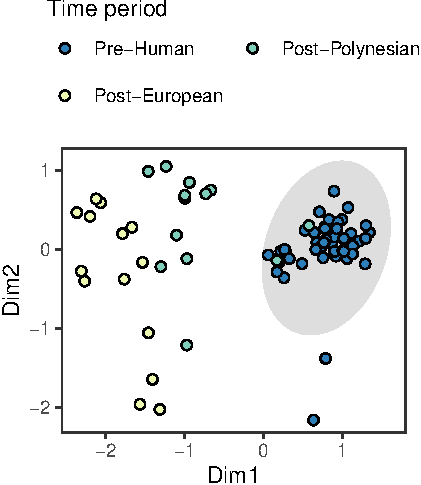
\includegraphics{Technical-supplement_files/figure-latex/boralDistPlot-1} \caption[Boral ordination with baseline ellipse shown in grey]{Boral ordination with baseline ellipse shown in grey.}\label{fig:boralDistPlot}
\end{marginfigure}

\hypertarget{distance-from-baseline-over-time---statistical-model}{%
\subsection{Distance from baseline over time - statistical
model}\label{distance-from-baseline-over-time---statistical-model}}

Overall, the ordination looks very similar to the NMDS ordination, so we
do not expect anything to change substantially with the models.

\begin{Shaded}
\begin{Highlighting}[]
\NormalTok{excludingPreHumanBoral }\OtherTok{\textless{}{-}}\NormalTok{ boralDistDF[}
\NormalTok{  boralDistDF}\SpecialCharTok{$}\NormalTok{period }\SpecialCharTok{!=} \StringTok{"Pre{-}Human"}\NormalTok{, ]}

\NormalTok{lmModEllipseBoral }\OtherTok{\textless{}{-}} \FunctionTok{lm}\NormalTok{(}\AttributeTok{data =}\NormalTok{ excludingPreHumanBoral, }
   \AttributeTok{formula =}\NormalTok{ distEllipse }\SpecialCharTok{\textasciitilde{}}\NormalTok{ YEAR }\SpecialCharTok{*}\NormalTok{ period,}
   \AttributeTok{na.action =} \StringTok{"na.fail"}\NormalTok{)}
\end{Highlighting}
\end{Shaded}

Here we see actually a difference between the NMDS and the boral
methods, in terms of what the best model is. With the boral method, we
see that the favoured model is one that includes year, time period, and
an interaction between the two. Using the NMDS method, we found the
favoured model included year only. Two key points here: the first is
that the in both cases the `other' model is very close to the favoured
model - delta AICc is 2 or less in both cases. Second, in this case you
might up the number of simulations that boral uses or try several
different random seeds (by setting the seed within the function) to see
if that affects results.

\begin{Shaded}
\begin{Highlighting}[]
\CommentTok{\# compare all subsets of global model }
\NormalTok{modTabBoral }\OtherTok{\textless{}{-}} \FunctionTok{dredge}\NormalTok{(lmModEllipseBoral)}
\NormalTok{knitr}\SpecialCharTok{::}\FunctionTok{kable}\NormalTok{(}\FunctionTok{model.sel}\NormalTok{(modTabBoral) }\SpecialCharTok{\%\textgreater{}\%}
               \FunctionTok{as.data.frame}\NormalTok{() }\SpecialCharTok{\%\textgreater{}\%}
           \FunctionTok{mutate}\NormalTok{(}\FunctionTok{across}\NormalTok{(}\FunctionTok{where}\NormalTok{(is.numeric), }
\NormalTok{                         \textbackslash{}(x) }\FunctionTok{sprintf}\NormalTok{(x, }
                         \AttributeTok{fmt =} \StringTok{"\%.3f"}\NormalTok{))) }\SpecialCharTok{\%\textgreater{}\%}
               \FunctionTok{rename}\NormalTok{(}\AttributeTok{Intercept =} \StringTok{\textasciigrave{}}\AttributeTok{(Intercept)}\StringTok{\textasciigrave{}}\NormalTok{), }
             \AttributeTok{digits =} \DecValTok{3}\NormalTok{,}
             \AttributeTok{caption =} \StringTok{"Model comparison {-} distance from baseline"}\NormalTok{)}
\end{Highlighting}
\end{Shaded}

\begin{longtable}[]{@{}
  >{\raggedright\arraybackslash}p{(\columnwidth - 18\tabcolsep) * \real{0.0411}}
  >{\raggedright\arraybackslash}p{(\columnwidth - 18\tabcolsep) * \real{0.1370}}
  >{\raggedright\arraybackslash}p{(\columnwidth - 18\tabcolsep) * \real{0.0959}}
  >{\raggedright\arraybackslash}p{(\columnwidth - 18\tabcolsep) * \real{0.0822}}
  >{\raggedright\arraybackslash}p{(\columnwidth - 18\tabcolsep) * \real{0.1644}}
  >{\raggedright\arraybackslash}p{(\columnwidth - 18\tabcolsep) * \real{0.0822}}
  >{\raggedright\arraybackslash}p{(\columnwidth - 18\tabcolsep) * \real{0.1096}}
  >{\raggedright\arraybackslash}p{(\columnwidth - 18\tabcolsep) * \real{0.0959}}
  >{\raggedright\arraybackslash}p{(\columnwidth - 18\tabcolsep) * \real{0.0959}}
  >{\raggedright\arraybackslash}p{(\columnwidth - 18\tabcolsep) * \real{0.0959}}@{}}
\caption{Model comparison - distance from baseline}\tabularnewline
\toprule\noalign{}
\begin{minipage}[b]{\linewidth}\raggedright
\end{minipage} & \begin{minipage}[b]{\linewidth}\raggedright
Intercept
\end{minipage} & \begin{minipage}[b]{\linewidth}\raggedright
period
\end{minipage} & \begin{minipage}[b]{\linewidth}\raggedright
YEAR
\end{minipage} & \begin{minipage}[b]{\linewidth}\raggedright
period:YEAR
\end{minipage} & \begin{minipage}[b]{\linewidth}\raggedright
df
\end{minipage} & \begin{minipage}[b]{\linewidth}\raggedright
logLik
\end{minipage} & \begin{minipage}[b]{\linewidth}\raggedright
AICc
\end{minipage} & \begin{minipage}[b]{\linewidth}\raggedright
delta
\end{minipage} & \begin{minipage}[b]{\linewidth}\raggedright
weight
\end{minipage} \\
\midrule\noalign{}
\endfirsthead
\toprule\noalign{}
\begin{minipage}[b]{\linewidth}\raggedright
\end{minipage} & \begin{minipage}[b]{\linewidth}\raggedright
Intercept
\end{minipage} & \begin{minipage}[b]{\linewidth}\raggedright
period
\end{minipage} & \begin{minipage}[b]{\linewidth}\raggedright
YEAR
\end{minipage} & \begin{minipage}[b]{\linewidth}\raggedright
period:YEAR
\end{minipage} & \begin{minipage}[b]{\linewidth}\raggedright
df
\end{minipage} & \begin{minipage}[b]{\linewidth}\raggedright
logLik
\end{minipage} & \begin{minipage}[b]{\linewidth}\raggedright
AICc
\end{minipage} & \begin{minipage}[b]{\linewidth}\raggedright
delta
\end{minipage} & \begin{minipage}[b]{\linewidth}\raggedright
weight
\end{minipage} \\
\midrule\noalign{}
\endhead
\bottomrule\noalign{}
\endlastfoot
8 & -10.592 & + & 0.006 & + & 5.000 & 5.771 & 1.315 & 0.000 & 0.662 \\
3 & -2.978 & NA & 0.003 & NA & 3.000 & 1.968 & 3.107 & 1.792 & 0.270 \\
4 & -3.049 & + & 0.003 & NA & 4.000 & 1.975 & 5.868 & 4.553 & 0.068 \\
2 & 1.964 & + & NA & NA & 3.000 & -12.723 & 32.489 & 31.174 & 0.000 \\
1 & 1.496 & NA & NA & NA & 2.000 & -25.472 & 55.444 & 54.128 & 0.000 \\
\end{longtable}

The model diagnostics look like some further work needs to be done! The
earliest two points have zero distance (no distance from baseline - they
fall within the ellipse on Fig. \ref{fig:boralDistPlot}) and are
affecting the slope of the line for the first time period. We could
(although don't) consider further whether we want the average rate of
change (as now) or the rate of change \emph{once the ecosystem starts to
be affected} i.e.~by excluding the earliest two points. Best to be
explicit either way. As for the NMDS model, the autocorrelation looks
fine.

\begin{Shaded}
\begin{Highlighting}[]
\CommentTok{\# favoured model}
\NormalTok{simpleLMBoral }\OtherTok{\textless{}{-}} \FunctionTok{lm}\NormalTok{(}\AttributeTok{data =}\NormalTok{ excludingPreHumanBoral, }
   \AttributeTok{formula =}\NormalTok{ distEllipse }\SpecialCharTok{\textasciitilde{}}\NormalTok{ YEAR }\SpecialCharTok{*}\NormalTok{ period)}

\CommentTok{\# set up 3 plots in a row}
\FunctionTok{par}\NormalTok{(}\AttributeTok{mfrow =} \FunctionTok{c}\NormalTok{(}\DecValTok{1}\NormalTok{, }\DecValTok{3}\NormalTok{))}

\CommentTok{\# first plot {-} raw vs fitted}
\FunctionTok{with}\NormalTok{(excludingPreHumanBoral, }
     \FunctionTok{plot}\NormalTok{(}\AttributeTok{x =}\NormalTok{ YEAR, }\AttributeTok{y =}\NormalTok{ distEllipse))}
\FunctionTok{title}\NormalTok{(}\AttributeTok{main =} \StringTok{"Fitted relationship to raw data"}\NormalTok{)}
\NormalTok{pp }\OtherTok{\textless{}{-}}\NormalTok{ excludingPreHumanBoral}\SpecialCharTok{$}\NormalTok{period}\SpecialCharTok{==}\StringTok{"Post{-}Polynesian"}
\FunctionTok{with}\NormalTok{(excludingPreHumanBoral[pp,], }
     \FunctionTok{lines}\NormalTok{(}\AttributeTok{x =}\NormalTok{ YEAR, }\AttributeTok{y =} \FunctionTok{fitted}\NormalTok{(simpleLMBoral)[pp]))}
\FunctionTok{with}\NormalTok{(excludingPreHumanBoral[}\SpecialCharTok{!}\NormalTok{pp,], }
     \FunctionTok{lines}\NormalTok{(}\AttributeTok{x =}\NormalTok{ YEAR, }\AttributeTok{y =} \FunctionTok{fitted}\NormalTok{(simpleLMBoral)[}\SpecialCharTok{!}\NormalTok{pp]))}

\CommentTok{\# second plot {-} residuals vs fitted}
\FunctionTok{plot}\NormalTok{(simpleLMBoral, }\AttributeTok{which =} \DecValTok{1}\NormalTok{,}
     \AttributeTok{caption =} \StringTok{""}\NormalTok{)}
\FunctionTok{title}\NormalTok{(}\AttributeTok{main =} \StringTok{"Residuals v fitted"}\NormalTok{)}

\CommentTok{\# third plot {-} autocorrelation.}
\FunctionTok{acf}\NormalTok{(}\FunctionTok{residuals}\NormalTok{(simpleLMBoral), }\AttributeTok{main =} \StringTok{"Autocorrelation plot"}\NormalTok{)}
\end{Highlighting}
\end{Shaded}

\begin{figure}
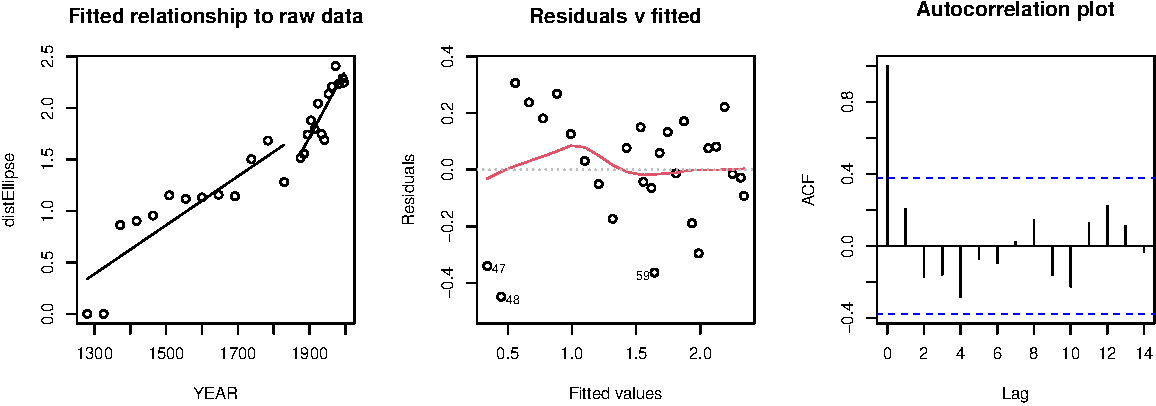
\includegraphics{Technical-supplement_files/figure-latex/unnamed-chunk-8-1} \caption[Model inspection]{Model inspection}\label{fig:unnamed-chunk-8}
\end{figure}

\begin{Shaded}
\begin{Highlighting}[]
\CommentTok{\# return to one plot per line}
\FunctionTok{par}\NormalTok{(}\AttributeTok{mfrow =} \FunctionTok{c}\NormalTok{(}\DecValTok{1}\NormalTok{, }\DecValTok{1}\NormalTok{))}
\end{Highlighting}
\end{Shaded}

Although we come to non-linear models (GAMs) later, there are several
other options: use a model accounting for temporal autocorrelation
(\texttt{gls}; above) or modify the year term (e.g.~include a quadratic
term, or similar).

\hypertarget{distance-from-start-point}{%
\section{Distance from start point}\label{distance-from-start-point}}

This approach is particularly useful where the pre-disturbance period is
unknown. For an example of published application, see Magurran,
Dornelas, Moyes, Gotelli, \& McGill
(\protect\hyperlink{ref-magurran_15_rapid}{2015}). Having decided on a
distance metric (e.g., Bray-Curtis, Jaccard), and having ensured that
the sample you wish to compare to is in the first row of your dataset,
we can calculate the distance from start point.

You can also calculate this yourself. It is easiest to do so by
converting the \texttt{distance} object created by \texttt{vegdist} (or
\texttt{dist}) to a matrix (\texttt{as.matrix()}), which for n samples,
will by a matrix of n rows and n columns, with 0 on the diagonal
(indicating that a sample is no different to itself). Here we give the
species data as the \texttt{rotonuiaha} dataframe, but remove the
\texttt{SITE}, \texttt{YEAR}, and \texttt{DEPTH} columns, as these are
not species data, but rather metadata. We include the metadata using the
\texttt{imps} dataframe we created earlier. The \texttt{idCol} (which
will be typically either a year or depth column) is given by
\texttt{YEAR} in our case and we have selected the Jaccard distance with
which to calculate ecological distance. We highlight that in our
dataset, it is already ordered deep-to-shallow, and therefore the year
84 AD (the first sample of the dataset) is in the first row. The
function also reports the value of the column that is used as the
reference level - please ensure you are happy with this.

\begin{Shaded}
\begin{Highlighting}[]
\NormalTok{pkStart }\OtherTok{\textless{}{-}} \FunctionTok{calculateDistanceStart}\NormalTok{(}
  \AttributeTok{speciesData =} \FunctionTok{decostand}\NormalTok{(}\FunctionTok{decostand}\NormalTok{(}
\NormalTok{    rotonuiaha[}\SpecialCharTok{!}\NormalTok{metaCols], }
    \StringTok{"total"}\NormalTok{), }\StringTok{"log"}\NormalTok{), }
  \AttributeTok{metaData =}\NormalTok{ imps,}
  \AttributeTok{idCol =} \StringTok{"YEAR"}\NormalTok{,}
  \AttributeTok{distMethod =} \StringTok{"jaccard"}\NormalTok{)}
\end{Highlighting}
\end{Shaded}

\begin{verbatim}
## [1] "Start/reference level value is 84.8340425531915 from column 'YEAR'"
\end{verbatim}

\texttt{pkStart} is the object returned by
\texttt{calculateDistanceStart} and has all the columns of the metadata
dataframe \texttt{imps}, and one extra column: the distance from start
(\texttt{dist\_jaccard}). The earliest sample will always have a
distance of 0 (we are comparing it to itself) and is removed using the
notation \texttt{pkStart{[}-1,\ {]}}, which removes the first row.

Before we get to running a model you can see that prior to human
arrival, distance from start averaged just below 0.5; increasing in the
post-Polynesian period and remaining high in the post-European period
(Fig. \ref{fig:distStartRaw}).

\begin{Shaded}
\begin{Highlighting}[]
\FunctionTok{ggplot}\NormalTok{(pkStart[ }\SpecialCharTok{{-}}\DecValTok{1}\NormalTok{, ], }\FunctionTok{aes}\NormalTok{(}\AttributeTok{x =}\NormalTok{ YEAR, }\AttributeTok{y =}\NormalTok{ dist\_jaccard)) }\SpecialCharTok{+}
  \FunctionTok{geom\_vline}\NormalTok{(}\AttributeTok{xintercept =} \DecValTok{1280}\NormalTok{, }\AttributeTok{linetype =} \StringTok{"dashed"}\NormalTok{,}
             \AttributeTok{colour =} \StringTok{"grey"}\NormalTok{) }\SpecialCharTok{+}
  \FunctionTok{geom\_vline}\NormalTok{(}\AttributeTok{xintercept =} \DecValTok{1840}\NormalTok{, }\AttributeTok{linetype =} \StringTok{"dashed"}\NormalTok{,}
             \AttributeTok{colour =} \StringTok{"grey"}\NormalTok{) }\SpecialCharTok{+}
  \FunctionTok{geom\_point}\NormalTok{(}\AttributeTok{shape =} \DecValTok{1}\NormalTok{) }\SpecialCharTok{+}
  \FunctionTok{geom\_line}\NormalTok{() }\SpecialCharTok{+} 
  \FunctionTok{coord\_cartesian}\NormalTok{(}\AttributeTok{ylim=} \FunctionTok{c}\NormalTok{(}\DecValTok{0}\NormalTok{, }\DecValTok{1}\NormalTok{)) }\SpecialCharTok{+}
  \FunctionTok{theme\_bw}\NormalTok{() }\SpecialCharTok{+}
  \FunctionTok{theme}\NormalTok{(}\AttributeTok{panel.grid =} \FunctionTok{element\_blank}\NormalTok{()) }\SpecialCharTok{+}
  \FunctionTok{labs}\NormalTok{(}\AttributeTok{x =} \StringTok{"Year"}\NormalTok{, }\AttributeTok{y =} \StringTok{"Ecological distance (Jaccard)"}\NormalTok{) }
\end{Highlighting}
\end{Shaded}

\begin{marginfigure}
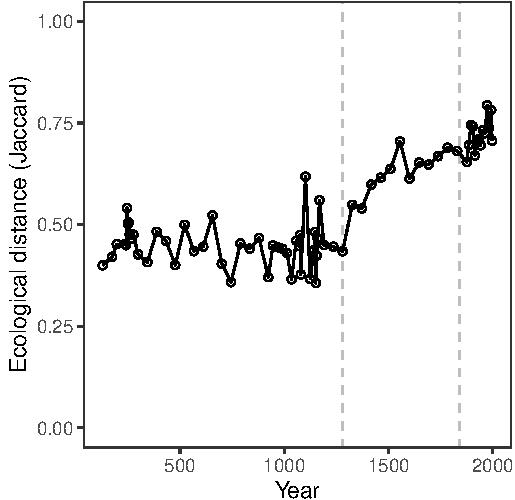
\includegraphics{Technical-supplement_files/figure-latex/distStartRaw-1} \caption[Distance from initial sample]{Distance from initial sample. Dashed lines indicate dates of Polynesian and Euro settlement}\label{fig:distStartRaw}
\end{marginfigure}

\hypertarget{gam-on-distance-from-start}{%
\subsection{GAM on distance from
start}\label{gam-on-distance-from-start}}

Note that there are a few points which look a bit squiffy on the
diagnostic plots. Without allowing the fitted smooth to `wiggle' wildly
to take these into account (or some other transformation of the data),
these will persist.

\begin{Shaded}
\begin{Highlighting}[]
\NormalTok{m2 }\OtherTok{\textless{}{-}} \FunctionTok{gamm}\NormalTok{(dist\_jaccard }\SpecialCharTok{\textasciitilde{}}  \FunctionTok{s}\NormalTok{(YEAR, }\AttributeTok{bs =} \StringTok{"cr"}\NormalTok{, }\AttributeTok{k =} \DecValTok{10}\NormalTok{),}
           \AttributeTok{correlation =} \FunctionTok{corCAR1}\NormalTok{(}\AttributeTok{form =} \SpecialCharTok{\textasciitilde{}}\NormalTok{ YEAR),}
           \AttributeTok{data =}\NormalTok{ pkStart[ }\SpecialCharTok{{-}}\DecValTok{1}\NormalTok{, ])}

\FunctionTok{par}\NormalTok{(}\AttributeTok{mfrow =} \FunctionTok{c}\NormalTok{(}\DecValTok{2}\NormalTok{,}\DecValTok{2}\NormalTok{))}

\FunctionTok{gam.check}\NormalTok{(m2}\SpecialCharTok{$}\NormalTok{gam)}
\end{Highlighting}
\end{Shaded}

\begin{figure}
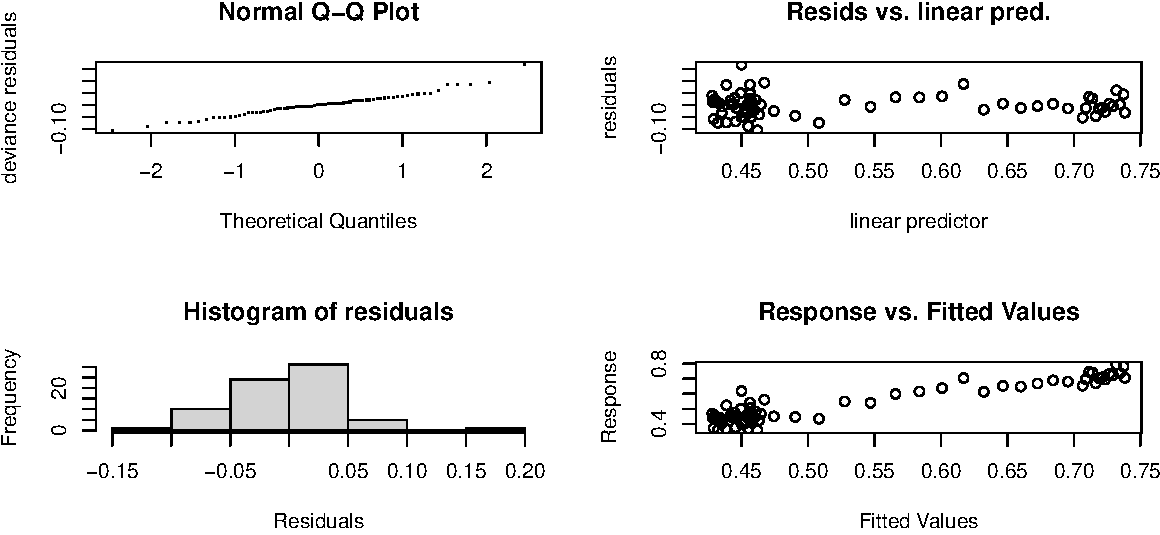
\includegraphics{Technical-supplement_files/figure-latex/distStartGAM-1} \caption[Diagnostic plots from GAMM model]{Diagnostic plots from GAMM model}\label{fig:distStartGAM}
\end{figure}

\begin{verbatim}
## 
## 'gamm' based fit - care required with interpretation.
## Checks based on working residuals may be misleading.
## Basis dimension (k) checking results. Low p-value (k-index<1) may
## indicate that k is too low, especially if edf is close to k'.
## 
##           k'  edf k-index p-value
## s(YEAR) 9.00 4.48    1.14    0.89
\end{verbatim}

\begin{Shaded}
\begin{Highlighting}[]
\FunctionTok{par}\NormalTok{(}\AttributeTok{mfrow =} \FunctionTok{c}\NormalTok{(}\DecValTok{1}\NormalTok{,}\DecValTok{1}\NormalTok{))}
\end{Highlighting}
\end{Shaded}

Below is the code to plot the raw and fitted data for Fig.
\ref{fig:distStartMod}.

\begin{Shaded}
\begin{Highlighting}[]
\FunctionTok{with}\NormalTok{(pkStart[ }\SpecialCharTok{{-}}\DecValTok{1}\NormalTok{, ], }\FunctionTok{plot}\NormalTok{(}\AttributeTok{x =}\NormalTok{ YEAR, }\AttributeTok{y =}\NormalTok{ dist\_jaccard,}
                          \AttributeTok{xlab =} \StringTok{"Year"}\NormalTok{,}
                          \AttributeTok{ylab =} \StringTok{"Distance"}\NormalTok{,}
                          \AttributeTok{col =} \StringTok{"grey50"}\NormalTok{))}
\FunctionTok{lines}\NormalTok{(}\AttributeTok{y =} \FunctionTok{predict}\NormalTok{(m2}\SpecialCharTok{$}\NormalTok{gam), }\AttributeTok{x =}\NormalTok{ pkStart[}\SpecialCharTok{{-}}\DecValTok{1}\NormalTok{, }\StringTok{"YEAR"}\NormalTok{],}
      \AttributeTok{col =} \StringTok{"darkorange"}\NormalTok{,}
      \AttributeTok{lwd =} \DecValTok{2}\NormalTok{)}
\end{Highlighting}
\end{Shaded}

\begin{marginfigure}
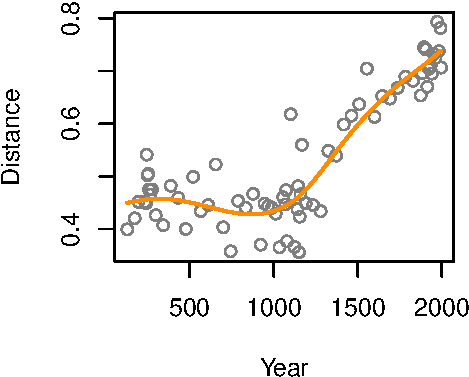
\includegraphics{Technical-supplement_files/figure-latex/distStartMod-1} \caption[Distance from initial sample - modelled and raw]{Distance from initial sample - modelled and raw}\label{fig:distStartMod}
\end{marginfigure}

\hypertarget{identifying-periods-of-rapid-change}{%
\subsection{Identifying periods of rapid
change}\label{identifying-periods-of-rapid-change}}

Here, we identify periods of rapid change, that is, where the first
derivative (i.e.~slope) of the fitted relationship from the GAMM is
significantly different to zero. This doesn't mean that there is a
difference from baseline - it is the rate of change in the distance that
is significant.

To calculate where the first derivative differs from zero, we use the
\texttt{gratia} package
(\protect\hyperlink{ref-simpson_2020_gratia}{Simpson, 2020}). We can
plot the derivative with confidence intervals (see Fig.
\ref{fig:calcDerivStart}). You can see that it only differs to zero at a
time period centred around 1500. This correlates with the increase in
distance-from-baseline beginning just prior and increasing rapidly
before plateauing.

\begin{Shaded}
\begin{Highlighting}[]
\NormalTok{newDat }\OtherTok{\textless{}{-}} \FunctionTok{data.frame}\NormalTok{(}\AttributeTok{YEAR =} \FunctionTok{seq}\NormalTok{(}
  \AttributeTok{from =} \FunctionTok{ceiling}\NormalTok{(}\FunctionTok{min}\NormalTok{(pkStart[}\SpecialCharTok{{-}}\DecValTok{1}\NormalTok{, }\StringTok{"YEAR"}\NormalTok{])),}
  \AttributeTok{to =} \FunctionTok{floor}\NormalTok{(}\FunctionTok{max}\NormalTok{(pkStart[}\SpecialCharTok{{-}}\DecValTok{1}\NormalTok{, }\StringTok{"YEAR"}\NormalTok{])),}
  \AttributeTok{by =} \DecValTok{1}\NormalTok{))}

\CommentTok{\# calculate the derivatives of the model}
\CommentTok{\# from gratia package}
\NormalTok{derivs }\OtherTok{\textless{}{-}} \FunctionTok{fderiv}\NormalTok{(m2, }\AttributeTok{newdata =}\NormalTok{ newDat) }
\CommentTok{\# calculate confidence intervals on the derivs}
\NormalTok{derivsCont }\OtherTok{\textless{}{-}} \FunctionTok{data.frame}\NormalTok{(newDat, }
                         \FunctionTok{confint}\NormalTok{(derivs, }
                                 \AttributeTok{type =} \StringTok{"simultaneous"}\NormalTok{))}


 \FunctionTok{ggplot}\NormalTok{(derivsCont, }\FunctionTok{aes}\NormalTok{(}\AttributeTok{x =}\NormalTok{ YEAR, }\AttributeTok{y =}\NormalTok{ est)) }\SpecialCharTok{+}
   \FunctionTok{geom\_hline}\NormalTok{(}\AttributeTok{yintercept =} \DecValTok{0}\NormalTok{, }\AttributeTok{linetype =} \StringTok{"dotted"}\NormalTok{) }\SpecialCharTok{+}
   \FunctionTok{geom\_line}\NormalTok{(}\FunctionTok{aes}\NormalTok{(}\AttributeTok{y =}\NormalTok{ lower),}\AttributeTok{linetype =} \StringTok{"dashed"}\NormalTok{) }\SpecialCharTok{+}
   \FunctionTok{geom\_line}\NormalTok{(}\FunctionTok{aes}\NormalTok{(}\AttributeTok{y =}\NormalTok{ upper),}\AttributeTok{linetype =} \StringTok{"dashed"}\NormalTok{) }\SpecialCharTok{+}
   
   \FunctionTok{geom\_point}\NormalTok{() }\SpecialCharTok{+}
   \FunctionTok{geom\_point}\NormalTok{(}\AttributeTok{data =}\NormalTok{ derivsCont  }\SpecialCharTok{\%\textgreater{}\%} 
                \FunctionTok{filter}\NormalTok{(}\SpecialCharTok{!}\NormalTok{(upper }\SpecialCharTok{\textgreater{}} \DecValTok{0} \SpecialCharTok{\&}\NormalTok{ lower }\SpecialCharTok{\textless{}} \DecValTok{0}\NormalTok{)),}
              \FunctionTok{aes}\NormalTok{(}\AttributeTok{colour =} \StringTok{"Slope different to zero"}\NormalTok{)) }\SpecialCharTok{+}
   \FunctionTok{theme\_bw}\NormalTok{() }\SpecialCharTok{+}
   \FunctionTok{scale\_colour\_manual}\NormalTok{(}
     \AttributeTok{values =} \FunctionTok{c}\NormalTok{(}\StringTok{"red2"}\NormalTok{, }\StringTok{"black"}\NormalTok{),}
     \AttributeTok{limits =} \FunctionTok{c}\NormalTok{(}\StringTok{"Slope different to zero"}\NormalTok{,}
                \StringTok{"Slope not different to zero"}\NormalTok{)) }\SpecialCharTok{+}
   \FunctionTok{theme}\NormalTok{(}\AttributeTok{legend.position =} \StringTok{"bottom"}\NormalTok{,}
         \AttributeTok{panel.grid =} \FunctionTok{element\_blank}\NormalTok{(),}
         \AttributeTok{legend.title =} \FunctionTok{element\_blank}\NormalTok{(),}
         \AttributeTok{legend.direction =} \StringTok{"vertical"}\NormalTok{)}
\end{Highlighting}
\end{Shaded}

\begin{marginfigure}
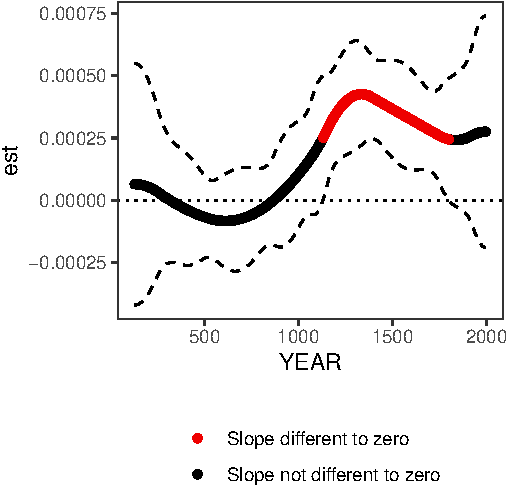
\includegraphics{Technical-supplement_files/figure-latex/calcDerivStart-1} \caption[First derivative with confidence intervals]{First derivative with confidence intervals}\label{fig:calcDerivStart}
\end{marginfigure}

This period of rapid change can be overlain on the previous figure,
which indicated change over time (Fig. \ref{fig:distStartRates}, below).

\begin{Shaded}
\begin{Highlighting}[]
\NormalTok{preds }\OtherTok{\textless{}{-}} \FunctionTok{data.frame}\NormalTok{(newDat, }
                    \AttributeTok{predicted =} \FunctionTok{predict}\NormalTok{(m2}\SpecialCharTok{$}\NormalTok{gam, }
                                        \AttributeTok{newdata =}\NormalTok{ newDat))}


\CommentTok{\# take the derivatives and }
\CommentTok{\# from: https://gist.github.com/gavinsimpson/ca18c9c789ef5237dbc6 }
\NormalTok{signifD }\OtherTok{\textless{}{-}} \ControlFlowTok{function}\NormalTok{(x, d, upper, lower, }\AttributeTok{eval =} \DecValTok{0}\NormalTok{) \{}
\NormalTok{  miss }\OtherTok{\textless{}{-}}\NormalTok{ upper }\SpecialCharTok{\textgreater{}}\NormalTok{ eval }\SpecialCharTok{\&}\NormalTok{ lower }\SpecialCharTok{\textless{}}\NormalTok{ eval}
\NormalTok{  incr }\OtherTok{\textless{}{-}}\NormalTok{ decr }\OtherTok{\textless{}{-}}\NormalTok{ x}
\NormalTok{  want }\OtherTok{\textless{}{-}}\NormalTok{ d }\SpecialCharTok{\textgreater{}}\NormalTok{ eval}
\NormalTok{  incr[}\SpecialCharTok{!}\NormalTok{want }\SpecialCharTok{|}\NormalTok{ miss] }\OtherTok{\textless{}{-}} \ConstantTok{NA}
\NormalTok{  want }\OtherTok{\textless{}{-}}\NormalTok{ d }\SpecialCharTok{\textless{}}\NormalTok{ eval}
\NormalTok{  decr[}\SpecialCharTok{!}\NormalTok{want }\SpecialCharTok{|}\NormalTok{ miss] }\OtherTok{\textless{}{-}} \ConstantTok{NA}
  \FunctionTok{list}\NormalTok{(}\AttributeTok{incr =}\NormalTok{ incr, }\AttributeTok{decr =}\NormalTok{ decr)}
\NormalTok{\}}

\NormalTok{sizes }\OtherTok{\textless{}{-}} \FunctionTok{signifD}\NormalTok{(derivsCont}\SpecialCharTok{$}\NormalTok{YEAR, }
                 \AttributeTok{d =}\NormalTok{ derivsCont}\SpecialCharTok{$}\NormalTok{est,}
                 \AttributeTok{upper =}\NormalTok{ derivsCont}\SpecialCharTok{$}\NormalTok{upper,}
                 \AttributeTok{lower =}\NormalTok{ derivsCont}\SpecialCharTok{$}\NormalTok{lower)}

\NormalTok{predSigs }\OtherTok{\textless{}{-}} \FunctionTok{data.frame}\NormalTok{(}
  \AttributeTok{year =}\NormalTok{ preds}\SpecialCharTok{$}\NormalTok{YEAR, }
  \AttributeTok{predicted =}\NormalTok{ preds}\SpecialCharTok{$}\NormalTok{predicted,}
  \AttributeTok{increasing =}\NormalTok{ sizes[[}\StringTok{"incr"}\NormalTok{]], }
  \AttributeTok{decreasing =}\NormalTok{ sizes[[}\StringTok{"decr"}\NormalTok{]]}
\NormalTok{  )}

\FunctionTok{ggplot}\NormalTok{(preds, }\FunctionTok{aes}\NormalTok{(}\AttributeTok{x =}\NormalTok{ YEAR, }\AttributeTok{y =}\NormalTok{ predicted)) }\SpecialCharTok{+}
  \FunctionTok{geom\_vline}\NormalTok{(}\AttributeTok{xintercept =} \DecValTok{1280}\NormalTok{, }\AttributeTok{linetype =} \StringTok{"dashed"}\NormalTok{,}
             \AttributeTok{colour =} \StringTok{"grey"}\NormalTok{) }\SpecialCharTok{+}
  \FunctionTok{geom\_vline}\NormalTok{(}\AttributeTok{xintercept =} \DecValTok{1840}\NormalTok{, }\AttributeTok{linetype =} \StringTok{"dashed"}\NormalTok{,}
             \AttributeTok{colour =} \StringTok{"grey"}\NormalTok{) }\SpecialCharTok{+}
  \FunctionTok{geom\_line}\NormalTok{() }\SpecialCharTok{+}
  \FunctionTok{theme\_bw}\NormalTok{() }\SpecialCharTok{+}
  \FunctionTok{geom\_path}\NormalTok{(}\AttributeTok{data=}\NormalTok{ predSigs,}
            \FunctionTok{aes}\NormalTok{(}\AttributeTok{x =}\NormalTok{ decreasing,}
                \AttributeTok{colour =} \StringTok{"Period of rapid change"}\NormalTok{),}
            \AttributeTok{size =} \DecValTok{2}\NormalTok{) }\SpecialCharTok{+}
  \FunctionTok{geom\_path}\NormalTok{(}\AttributeTok{data=}\NormalTok{ predSigs,}
            \FunctionTok{aes}\NormalTok{(}\AttributeTok{x =}\NormalTok{ increasing,}
                \AttributeTok{colour =} \StringTok{"Period of rapid change"}\NormalTok{),}
            \AttributeTok{size =} \DecValTok{2}\NormalTok{) }\SpecialCharTok{+}
  \FunctionTok{labs}\NormalTok{(}\AttributeTok{x =} \StringTok{"Year"}\NormalTok{, }\AttributeTok{y =} \StringTok{"Distance from start"}\NormalTok{) }\SpecialCharTok{+}
  \FunctionTok{scale\_colour\_manual}\NormalTok{(}\AttributeTok{values =} \StringTok{"red2"}\NormalTok{) }\SpecialCharTok{+}
  \FunctionTok{geom\_point}\NormalTok{(}\AttributeTok{data =}\NormalTok{ pkStart[ }\SpecialCharTok{{-}}\DecValTok{1}\NormalTok{, ], }
             \FunctionTok{aes}\NormalTok{(}\AttributeTok{x =}\NormalTok{ YEAR, }\AttributeTok{y =}\NormalTok{ dist\_jaccard),}
             \AttributeTok{shape =} \DecValTok{1}\NormalTok{) }\SpecialCharTok{+}
  \FunctionTok{theme}\NormalTok{(}\AttributeTok{legend.title =} \FunctionTok{element\_blank}\NormalTok{(),}
        \AttributeTok{legend.position =} \FunctionTok{c}\NormalTok{(}\FloatTok{0.02}\NormalTok{, }\FloatTok{0.98}\NormalTok{),}
        \AttributeTok{legend.justification =} \FunctionTok{c}\NormalTok{(}\DecValTok{0}\NormalTok{, }\DecValTok{1}\NormalTok{),}
        \AttributeTok{panel.grid =} \FunctionTok{element\_blank}\NormalTok{())}
\end{Highlighting}
\end{Shaded}

\begin{figure}
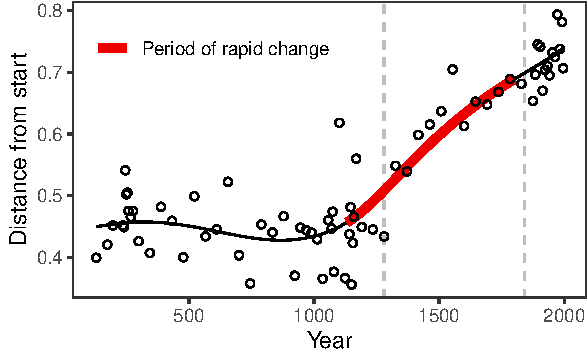
\includegraphics{Technical-supplement_files/figure-latex/distStartRates-1} \caption[GAMM model with period of rapid change highlighted in red]{GAMM model with period of rapid change highlighted in red}\label{fig:distStartRates}
\end{figure}

\hypertarget{principal-curves}{%
\section{Principal curves}\label{principal-curves}}

Principal curves are an ordination technique which are a one-dimensional
curve fitted through multidimensional datasets\footnote{see excellent
  blog post by Gavin Simpson
  \href{https://www.fromthebottomoftheheap.net/2014/01/09/pcurve-part-2/}{here}}.
Here we fit one to the Rotonuiaha site. We transform the data using a
Hellinger transformation (see \texttt{?decostand} for details).

\begin{Shaded}
\begin{Highlighting}[]
\NormalTok{prc1 }\OtherTok{\textless{}{-}} \FunctionTok{prcurve}\NormalTok{(}\FunctionTok{decostand}\NormalTok{(rotonuiaha[}\SpecialCharTok{!}\NormalTok{metaCols], }
                          \StringTok{"hellinger"}\NormalTok{), }
                \AttributeTok{trace =} \ConstantTok{FALSE}\NormalTok{, }\AttributeTok{plotit =} \ConstantTok{FALSE}\NormalTok{,  }
                \AttributeTok{maxit =} \DecValTok{500}\NormalTok{)}

\NormalTok{prc1}
\end{Highlighting}
\end{Shaded}

\begin{verbatim}
## 
##  Principal Curve Fitting
## 
## Call: prcurve(X = decostand(rotonuiaha[!metaCols], "hellinger"), maxit
## = 500, trace = FALSE, plotit = FALSE)
## 
## Algorithm converged after 5 iterations
## 
##           SumSq Proportion
## Total     20.25       1.00
## Explained 15.19       0.75
## Residual   5.06       0.25
## 
## Fitted curve uses 541.194 degrees of freedom.
\end{verbatim}

\begin{Shaded}
\begin{Highlighting}[]
\NormalTok{prcurveScores }\OtherTok{\textless{}{-}} \FunctionTok{data.frame}\NormalTok{(imps, }\FunctionTok{scores}\NormalTok{(prc1)) }
\end{Highlighting}
\end{Shaded}

The principal curve scores in raw form indicate that there was periods
of rapid change after Polynesian and European settlement - and
substantial, but short-lived, change at the time of the Taupō eruption
(Fig. \ref{fig:prRawFitPlot}).

\begin{Shaded}
\begin{Highlighting}[]
\FunctionTok{ggplot}\NormalTok{(prcurveScores, }
       \FunctionTok{aes}\NormalTok{(}\AttributeTok{x =}\NormalTok{ YEAR, }\AttributeTok{y =}\NormalTok{ PrC)) }\SpecialCharTok{+}
  \FunctionTok{geom\_vline}\NormalTok{(}\AttributeTok{xintercept =} \DecValTok{232}\NormalTok{, }\AttributeTok{linetype =} \StringTok{"dotdash"}\NormalTok{,}
             \AttributeTok{colour =} \StringTok{"darkorange"}\NormalTok{) }\SpecialCharTok{+}
  \FunctionTok{geom\_vline}\NormalTok{(}\AttributeTok{xintercept =} \DecValTok{1280}\NormalTok{, }\AttributeTok{linetype =} \StringTok{"dashed"}\NormalTok{,}
             \AttributeTok{colour =} \StringTok{"grey50"}\NormalTok{) }\SpecialCharTok{+}
  \FunctionTok{geom\_vline}\NormalTok{(}\AttributeTok{xintercept =} \DecValTok{1840}\NormalTok{, }\AttributeTok{linetype =} \StringTok{"dashed"}\NormalTok{,}
             \AttributeTok{colour =} \StringTok{"grey50"}\NormalTok{) }\SpecialCharTok{+}
  \FunctionTok{geom\_point}\NormalTok{(}\AttributeTok{shape =} \DecValTok{16}\NormalTok{) }\SpecialCharTok{+} 
  \FunctionTok{geom\_line}\NormalTok{() }\SpecialCharTok{+}
  \FunctionTok{theme\_bw}\NormalTok{()  }\SpecialCharTok{+} 
  \FunctionTok{theme}\NormalTok{(}\AttributeTok{panel.grid =} \FunctionTok{element\_blank}\NormalTok{())}
\end{Highlighting}
\end{Shaded}

\begin{marginfigure}
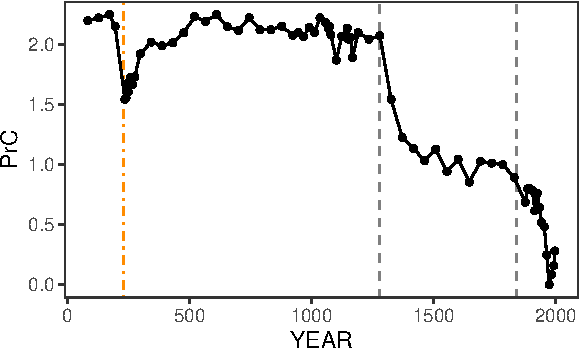
\includegraphics{Technical-supplement_files/figure-latex/prRawFitPlot-1} \caption[Principal curve scores over time]{Principal curve scores over time. Orange line indicates the Taupō eruption.}\label{fig:prRawFitPlot}
\end{marginfigure}

We now use a gam to test for where periods of rapid change occur. This
follows the same process as above for distance from start.

\begin{Shaded}
\begin{Highlighting}[]
\NormalTok{prcurveScores}\SpecialCharTok{$}\NormalTok{year }\OtherTok{\textless{}{-}} \FunctionTok{round}\NormalTok{(prcurveScores}\SpecialCharTok{$}\NormalTok{YEAR, }\DecValTok{0}\NormalTok{)}

\NormalTok{prGamm }\OtherTok{\textless{}{-}} \FunctionTok{gamm}\NormalTok{(PrC }\SpecialCharTok{\textasciitilde{}}  \FunctionTok{s}\NormalTok{(YEAR, }\AttributeTok{bs =} \StringTok{"cr"}\NormalTok{, }\AttributeTok{k =} \DecValTok{20}\NormalTok{),}
               \AttributeTok{correlation =} \FunctionTok{corCAR1}\NormalTok{(}\AttributeTok{form =} \SpecialCharTok{\textasciitilde{}}\NormalTok{ year),}
               \CommentTok{\# method = "REML",}
               \AttributeTok{data =}\NormalTok{ prcurveScores)}

\FunctionTok{par}\NormalTok{(}\AttributeTok{mfrow =} \FunctionTok{c}\NormalTok{(}\DecValTok{2}\NormalTok{,}\DecValTok{2}\NormalTok{))}
\FunctionTok{gam.check}\NormalTok{(prGamm}\SpecialCharTok{$}\NormalTok{gam)}
\end{Highlighting}
\end{Shaded}

\begin{figure}
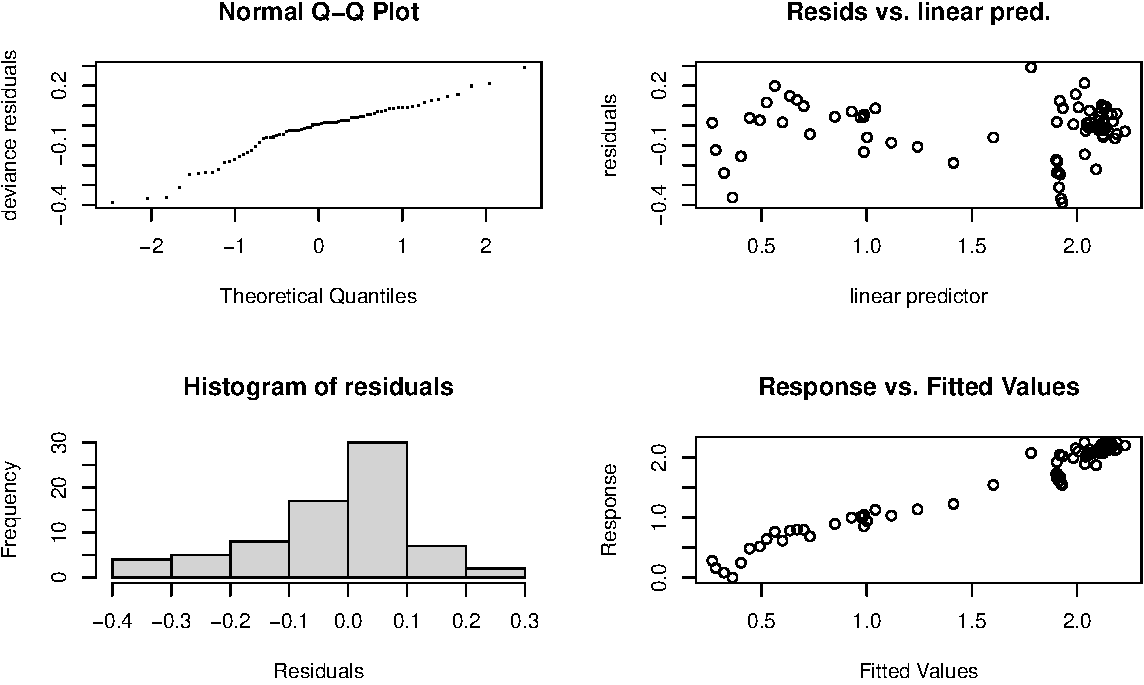
\includegraphics{Technical-supplement_files/figure-latex/gamprc-1} \caption[PrC GAMM diagnostics]{PrC GAMM diagnostics}\label{fig:gamprc}
\end{figure}

\begin{verbatim}
## 
## 'gamm' based fit - care required with interpretation.
## Checks based on working residuals may be misleading.
## Basis dimension (k) checking results. Low p-value (k-index<1) may
## indicate that k is too low, especially if edf is close to k'.
## 
##           k'  edf k-index p-value    
## s(YEAR) 19.0  8.9    0.45  <2e-16 ***
## ---
## Signif. codes:  0 '***' 0.001 '**' 0.01 '*' 0.05 '.' 0.1 ' ' 1
\end{verbatim}

\begin{Shaded}
\begin{Highlighting}[]
\FunctionTok{par}\NormalTok{(}\AttributeTok{mfrow =} \FunctionTok{c}\NormalTok{(}\DecValTok{1}\NormalTok{,}\DecValTok{1}\NormalTok{))}
\end{Highlighting}
\end{Shaded}

\begin{Shaded}
\begin{Highlighting}[]
\NormalTok{GAMMsterPlot }\OtherTok{\textless{}{-}} \FunctionTok{ggplot}\NormalTok{(prcurveScores, }\FunctionTok{aes}\NormalTok{(}\AttributeTok{x =}\NormalTok{ year, }\AttributeTok{y =}\NormalTok{ PrC)) }\SpecialCharTok{+}
  \FunctionTok{geom\_point}\NormalTok{() }\SpecialCharTok{+}
  \FunctionTok{theme\_bw}\NormalTok{() }\SpecialCharTok{+} 
  \FunctionTok{geom\_line}\NormalTok{(}\AttributeTok{y =} \FunctionTok{fitted}\NormalTok{(prGamm}\SpecialCharTok{$}\NormalTok{gam), }\AttributeTok{colour =} \StringTok{"red2"}\NormalTok{)}
\end{Highlighting}
\end{Shaded}

We see that the GAMM model is a poor fit for the period of rapid change
around the Taupō eruption; we can try a GAM model with adaptive splines
to address this.

\begin{Shaded}
\begin{Highlighting}[]
\NormalTok{prGam }\OtherTok{\textless{}{-}} \FunctionTok{gam}\NormalTok{(PrC }\SpecialCharTok{\textasciitilde{}}  \FunctionTok{s}\NormalTok{(year, }\AttributeTok{bs =} \StringTok{"ad"}\NormalTok{, }\AttributeTok{k =} \DecValTok{20}\NormalTok{),}
               \CommentTok{\# correlation = corCAR1(form = \textasciitilde{} year),}
               \AttributeTok{method =} \StringTok{"REML"}\NormalTok{,}
               \AttributeTok{data =}\NormalTok{ prcurveScores)}



\NormalTok{GAMsterPlot }\OtherTok{\textless{}{-}} \FunctionTok{ggplot}\NormalTok{(prcurveScores, }\FunctionTok{aes}\NormalTok{(}\AttributeTok{x =}\NormalTok{ year, }\AttributeTok{y =}\NormalTok{ PrC)) }\SpecialCharTok{+}
  \FunctionTok{geom\_point}\NormalTok{() }\SpecialCharTok{+}
  \FunctionTok{theme\_bw}\NormalTok{() }\SpecialCharTok{+} 
  \FunctionTok{geom\_line}\NormalTok{(}\AttributeTok{y =} \FunctionTok{fitted}\NormalTok{(prGam), }\AttributeTok{colour =} \StringTok{"royalblue"}\NormalTok{)}

\FunctionTok{grid.arrange}\NormalTok{(GAMMsterPlot }\SpecialCharTok{+} \FunctionTok{ggtitle}\NormalTok{(}\StringTok{"(A) GAMM plot"}\NormalTok{), }
\NormalTok{             GAMsterPlot }\SpecialCharTok{+} \FunctionTok{ggtitle}\NormalTok{(}\StringTok{"(B) GAM plot"}\NormalTok{),}
             \AttributeTok{nrow =} \DecValTok{1}\NormalTok{)}
\end{Highlighting}
\end{Shaded}

\begin{figure}
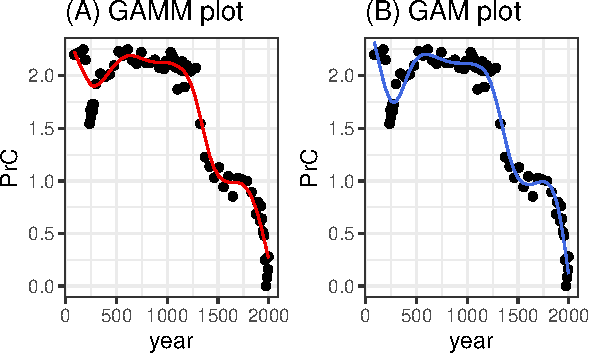
\includegraphics{Technical-supplement_files/figure-latex/unnamed-chunk-11-1} \caption[PrC (a) GAMM and (b) GAM with adaptive spline - raw scores and fitted relationships]{PrC (a) GAMM and (b) GAM with adaptive spline - raw scores and fitted relationships.}\label{fig:unnamed-chunk-11}
\end{figure}

\begin{Shaded}
\begin{Highlighting}[]
\NormalTok{mod }\OtherTok{\textless{}{-}}\NormalTok{ prGamm}\SpecialCharTok{$}\NormalTok{gam}

\NormalTok{pcData }\OtherTok{\textless{}{-}} \FunctionTok{data.frame}\NormalTok{(}
  \AttributeTok{YEAR =} \FunctionTok{seq}\NormalTok{(}\AttributeTok{from =} \FunctionTok{ceiling}\NormalTok{(}\FunctionTok{min}\NormalTok{(imps}\SpecialCharTok{$}\NormalTok{YEAR)),}
             \AttributeTok{to =} \FunctionTok{floor}\NormalTok{(}\FunctionTok{max}\NormalTok{(imps}\SpecialCharTok{$}\NormalTok{YEAR)),}
             \AttributeTok{by =} \DecValTok{1}\NormalTok{)}
\NormalTok{)}
\NormalTok{predPC }\OtherTok{\textless{}{-}} \FunctionTok{data.frame}\NormalTok{(pcData, }
                     \AttributeTok{predicted =} \FunctionTok{predict}\NormalTok{(mod, }
                                         \AttributeTok{newdata =}\NormalTok{ pcData))}

\NormalTok{derivsPC }\OtherTok{\textless{}{-}} \FunctionTok{fderiv}\NormalTok{(mod, }\AttributeTok{newdata =}\NormalTok{ pcData) }
\NormalTok{derivsContPC }\OtherTok{\textless{}{-}} \FunctionTok{data.frame}\NormalTok{(pcData, }
                           \FunctionTok{confint}\NormalTok{(derivsPC, }
                                   \AttributeTok{type =} \StringTok{"simultaneous"}\NormalTok{))}


\NormalTok{sizesPC }\OtherTok{\textless{}{-}} \FunctionTok{signifD}\NormalTok{(derivsContPC}\SpecialCharTok{$}\NormalTok{YEAR, }
                 \AttributeTok{d =}\NormalTok{ derivsContPC}\SpecialCharTok{$}\NormalTok{est,}
        \AttributeTok{upper =}\NormalTok{ derivsContPC}\SpecialCharTok{$}\NormalTok{upper,}
        \AttributeTok{lower =}\NormalTok{ derivsContPC}\SpecialCharTok{$}\NormalTok{lower)}


\NormalTok{predSigsPC }\OtherTok{\textless{}{-}} \FunctionTok{data.frame}\NormalTok{(}
  \AttributeTok{YEAR =}\NormalTok{ predPC}\SpecialCharTok{$}\NormalTok{YEAR, }
  \AttributeTok{predicted =}\NormalTok{ predPC}\SpecialCharTok{$}\NormalTok{predicted,}
  \AttributeTok{increasing =}\NormalTok{ sizesPC[[}\DecValTok{1}\NormalTok{]], }
  \AttributeTok{decreasing =}\NormalTok{ sizesPC[[}\DecValTok{2}\NormalTok{]]}
\NormalTok{  )}

\FunctionTok{ggplot}\NormalTok{(predPC, }\FunctionTok{aes}\NormalTok{(}\AttributeTok{x=}\NormalTok{ YEAR, }\AttributeTok{y =}\NormalTok{ predicted)) }\SpecialCharTok{+} 
  \FunctionTok{geom\_vline}\NormalTok{(}\AttributeTok{xintercept =} \DecValTok{232}\NormalTok{, }
             \AttributeTok{linetype =} \StringTok{"dotdash"}\NormalTok{,}
             \AttributeTok{col =} \StringTok{"darkorange"}\NormalTok{) }\SpecialCharTok{+}
    \FunctionTok{geom\_vline}\NormalTok{(}\AttributeTok{xintercept =} \DecValTok{1280}\NormalTok{, }
             \AttributeTok{linetype =} \StringTok{"dashed"}\NormalTok{,}
             \AttributeTok{col =} \StringTok{"grey50"}\NormalTok{) }\SpecialCharTok{+}
    \FunctionTok{geom\_vline}\NormalTok{(}\AttributeTok{xintercept =} \DecValTok{1840}\NormalTok{, }
             \AttributeTok{linetype =} \StringTok{"dashed"}\NormalTok{,}
             \AttributeTok{col =} \StringTok{"grey50"}\NormalTok{) }\SpecialCharTok{+}
  \FunctionTok{geom\_point}\NormalTok{(}\AttributeTok{data =}\NormalTok{ prcurveScores, }\FunctionTok{aes}\NormalTok{(}\AttributeTok{y =}\NormalTok{ PrC),}
             \AttributeTok{shape =} \DecValTok{1}\NormalTok{) }\SpecialCharTok{+}
  \FunctionTok{geom\_path}\NormalTok{() }\SpecialCharTok{+}
  \FunctionTok{geom\_path}\NormalTok{(}\AttributeTok{data=}\NormalTok{ predSigsPC, }\FunctionTok{aes}\NormalTok{(}\AttributeTok{x =}\NormalTok{ decreasing),}
            \AttributeTok{size =} \DecValTok{2}\NormalTok{, }\AttributeTok{colour =} \StringTok{"red2"}\NormalTok{) }\SpecialCharTok{+} 
  \FunctionTok{geom\_path}\NormalTok{(}\AttributeTok{data=}\NormalTok{ predSigsPC, }\FunctionTok{aes}\NormalTok{(}\AttributeTok{x =}\NormalTok{ increasing),}
            \AttributeTok{size =} \DecValTok{2}\NormalTok{, }\AttributeTok{colour =} \StringTok{"red2"}\NormalTok{) }\SpecialCharTok{+} 
  \FunctionTok{theme\_bw}\NormalTok{() }\SpecialCharTok{+}
  \FunctionTok{theme}\NormalTok{(}\AttributeTok{panel.grid =} \FunctionTok{element\_blank}\NormalTok{())}
\end{Highlighting}
\end{Shaded}

\begin{marginfigure}
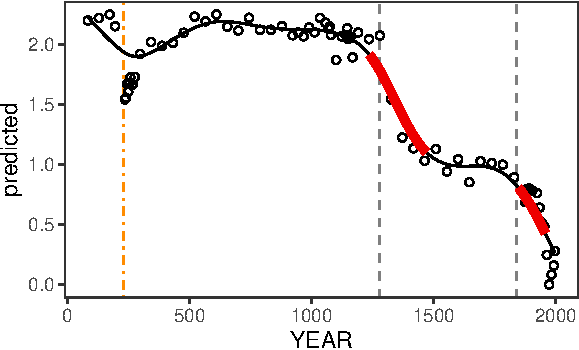
\includegraphics{Technical-supplement_files/figure-latex/gamRates-1} \caption[Periods of rapid change modelled using GAMM and PrC scores]{Periods of rapid change modelled using GAMM and PrC scores}\label{fig:gamRates}
\end{marginfigure}

You'll note that the Taupō volcanic eruption eruption of 232 AD (orange
dashed lines) is reflected to an extent by the fitted gam relationship;
while the change following human settlement is prolonged and substantial
and reflected in the rapid rates of change found following the model
(Fig. \ref{fig:gamRates}). A gam and a thin plate spline was able to
derive a better fit to the data (code not shown).

\hypertarget{conclusions}{%
\section{Conclusions}\label{conclusions}}

This supplement has set out the methods by which one can calculate
distance from baseline and change over time, and testing (a) whether a
priori defined periods differ in their distance from baseline and (b)
whether (and where) there are rapid periods of change.

\clearpage

\hypertarget{references}{%
\section*{References}\label{references}}
\addcontentsline{toc}{section}{References}

\hypertarget{refs}{}
\begin{CSLReferences}{0}{5}
\leavevmode\vadjust pre{\hypertarget{ref-burge_2022_baselines}{}}%
Burge, O. R. (2022). Baselines: {A} package to calculate baselines from
multivariate data.
doi:\href{https://doi.org/10.5281/zenodo.6420020}{10.5281/zenodo.6420020}

\leavevmode\vadjust pre{\hypertarget{ref-burge_2022_incorporating}{}}%
Burge, O. R., Richardson, S. J., Wood, J. R., \& Wilmshurst, J. M.
(2023). A guide to assess distance from ecological baselines and change
over time in palaeoecological records. \emph{The Holocene},
\emph{33}(8), 905--917.
doi:\href{https://doi.org/10.1177/09596836231169986}{10.1177/09596836231169986}

\leavevmode\vadjust pre{\hypertarget{ref-hui16_boral}{}}%
Hui, F. K. C. (2016). Boral \textendash{} bayesian ordination and
regression analysis of multivariate abundance data in {R}. \emph{Methods
in Ecology and Evolution}, \emph{7}(6), 744--750.
doi:\href{https://doi.org/10.1111/2041-210X.12514}{10.1111/2041-210X.12514}

\leavevmode\vadjust pre{\hypertarget{ref-magurran_15_rapid}{}}%
Magurran, A. E., Dornelas, M., Moyes, F., Gotelli, N. J., \& McGill, B.
(2015). Rapid biotic homogenization of marine fish assemblages.
\emph{Nature Communications}, \emph{6}, ncomms9405.
doi:\href{https://doi.org/10.1038/ncomms9405}{10.1038/ncomms9405}

\leavevmode\vadjust pre{\hypertarget{ref-oksanen_2019_vegan}{}}%
Oksanen, J., Blanchet, F. G., Friendly, M., Kindt, R., Legendre, P.,
McGlinn, D., Minchin, P. R., O'Hara, R. B., \ldots{} Wagner, H. (2019).
Vegan: {Community} ecology package. {R} package version 2.5-6.

\leavevmode\vadjust pre{\hypertarget{ref-simpson_2020_gratia}{}}%
Simpson, G. L. (2020). Gratia: Graceful {`ggplot'}-{Based} graphics and
other functions for {GAMs} fitted using {`mgcv'}. {R} package version
0.3.0.

\leavevmode\vadjust pre{\hypertarget{ref-wickham_2016_ggplot2}{}}%
Wickham, H. (2016). \emph{Ggplot2: Elegant graphics for data analysis}.
{New York}: {Springer-Verlag}.

\leavevmode\vadjust pre{\hypertarget{ref-wilmshurst_96_forest}{}}%
Wilmshurst, J. M., \& McGlone, M. S. (1996). Forest disturbance in the
central {North Island}, {New Zealand}, following the 1850 {BP Taupo}
eruption. \emph{The Holocene}, \emph{6}(4), 399--411.
doi:\href{https://doi.org/10.1177/095968369600600402}{10.1177/095968369600600402}

\end{CSLReferences}



\end{document}
